\chapter{Generating Code for Graph Programs on a Manycore Architecture}\label{gen:sec:graphitbackend}
\markboth{Generating Code for Manycore Graph Programs}{Generating Code for Manycore Graph Programs}

\introOverviewFigure

%\todo{intro paragraph to discuss the problem with graph processing again?/contextualize after background and related work?}
To harness the benefits of manycore architectures and reduce programming complexity, we propose a code generation backend for GraphIt, a flexible domain-specific language (DSL) for graph computations~\cite{zhang2018graphit}. 
This backend generates code targetting the representative manycore architecture described in \ref{gen:sec:background}.
We use this new backend to explore several optimizations on three well-known graph benchmarks.
Our evaluation shows that our GraphIt backend achieves a maximum of 467.1 million traversed edges per second (MTEPS) and on average achieves 252.7 MTEPS across all input graphs and benchmarks studied. 
We find that our optimizations achieve a maximum speedup of 2.1$\times$ and an average speedup of 1.16$\times$ over naive manycore implementations.
An overview of our approach is shown in Figure~\ref{pap:generals:sec:intro:fig:overview}.

This section makes the following contributions:
\begin{itemize}
    \item A backend for the GraphIt domain-specific language~\cite{zhang2018graphit} that targets a prototypical manycore architecture.
    \item A performance study of different graph processing optimizations on manycore architectures which shows a maximum speedup of 2.1$\times$.
    \item An evaluation of our GraphIt backend that shows that it achieves a maximum of 467.1 MTEPS.
\end{itemize}

The rest of this section is organized as follows:
% We introduce manycore architectures and describe our target architecture in Section~\ref{pap:oopsla2020:sec:architecture}.
% We provide background on the GraphIt DSL in
% Section~\ref{pap:oopsla2020:sec:graphit}. 
In Subsections~\ref{sec:method} and ~\ref{sec:method:sub:baseline}, I describe how we compile GraphIt programs to the manycore architecture and demonstrate the scheduling optimizations that we explore.
I present and discuss the performance results of our compiled graph workloads in Subsection~\ref{sec:eval} and Subsection~\ref{sec:discussion}.
%We cover related work in Section~\ref{sec:related}.
I end with conclusions in Subsection~\ref{sec:concl}.

%subsections:
%\newcommand{\manycoreArchFigure}{
\begin{figure}[t]
    \centering
    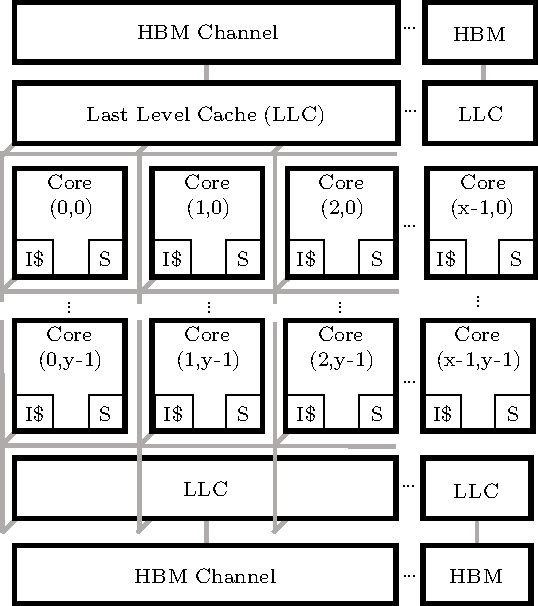
\includegraphics[scale=0.8]{graphit-figures/manycore-arch.pdf}
    \caption{Block diagram of the general manycore architecture targeted in
      this thesis. A 2D-Mesh Network-on-Chip connects general-purpose
      computation cores and Last Level Caches (LLC). Each LLC connects to a single
      independent High-Bandwidth Memory (HBM) channel.}
    \label{pap:generals:sec:architecture:fig:hbarch}
\end{figure}
}
\section{Manycore Architectures} \label{pap:generals:sec:architecture}
Manycore architectures provide thread-level parallelism and flexibility with hundreds to thousands of general-purpose cores~\cite{ramey2011tilera, davidson2018celerity, gwennap2011adapteva, agathos2015parallela, taylor2004raw}.
Cores are arranged in two-dimensional arrays and interconnected with mesh-style networks for communication.
This network of cores is surrounded by multiple channels of memory to provide sufficient bandwidth and parallelism to sustain computation.
Cores within the architecture communicate explicitly through memory~\cite{davidson2018celerity} or message passing \cite{gwennap2011adapteva}, implicitly through coherence protocols~\cite{ramey2011tilera}, or both using inter-core result networks \cite{taylor2004raw}.
Communication allows cores to cooperate and solve large parallel tasks.
The quantity of cores and diverse communication patterns means that manycore architectures provide a flexible parallel computation fabric that can be tailored to fit application requirements or the structure of graph input data \cite{lumsdaine2007challenges}.

In this section, I describe a representative manycore architecture that we use to evaluate our code generator.
The cores are tiny, performance-optimized scalar cores that implement a RISC-V instruction set.
Each core has a software-managed scratchpad memory for low-latency storage and inter-thread communication.
Data cache lines do not move between cores, eliminating coherence overhead and false sharing.
The memory system is designed to expose memory parallelism and bandwidth to service memory requests from hundreds of concurrent threads.
This architecture is emblematic of Single Program Multiple Data (SPMD) parallel machines where collections of cores are loaded with the same program, but each core computes on different input data.

This section provides a overview of the target manycore
architecture depicted in
Figure~\ref{pap:generals:sec:architecture:fig:hbarch}. The
architecture is composed of efficient general-purpose processor cores,
Last Level Caches (LLCs), a 2D-Mesh Network on Chip, and High-Bandwidth
Memory (HBM) channels.
%% Fluff -M
%The system is designed for efficient
%computation of general-purpose scientific, graph, and machine-learning
%workloads that can exploit the unprecedented memory-level parallelism
%provided by the independent cores, caches, and HBM channels.

\manycoreArchFigure

\subsection{Network-On-Chip}
Communication is provided by a 2D-Mesh Network-on-Chip (NoC) that
interconnects Last Level Caches and general-purpose cores. The
NoC supports point-to-point communication between endpoints using
shared memory. All addressable endpoints within the network are
assigned a unique global address range. This provides a PGAS-like
(Partitioned Global Address Space) memory model for execution.

\subsection{Memory System}
The manycore's memory system is designed to provide the high-bandwidth memory-level parallelism required by manycore
architectures. The memory system has four hierarchy levels:
High-Bandwidth Memory (HBM), Last Level Cache (LLC), core-remote
scratchpad (S), and core-local scratchpad (S). Each level is designed
to exploit memory parallelism and exposes a trade-off between latency,
capacity, as shown in
Figure~\ref{pap:generals:sec:architecture:fig:hbarch}.

Manycore architectures require many high-bandwidth and independent
memory channels to supply data for computation, so we use
second-generation High Bandwidth Memory (HBM, or HBM2). HBM provides
two sources of memory-level parallelism: First, HBM provides
channel-level parallelism with 8 independent physical channel
interfaces per chiplet. Each channel has a maximum data transfer rate of 32
GB/s. Second, HBM provides bank-level parallelism through pipelining
commands. Commands for opening/closing banks and reading data are
overlapped to hide the latency of long-running commands. Compared to
traditional SDRAM/DIMM-based devices, HBM provides more bandwidth
per-package and parallelism and is ideal for manycore
architectures, but performance depends on exploiting channel-level and
bank-level parallelism.

The banked Last Level Caches (LLC) shown in 
Figure~\ref{pap:generals:sec:architecture:fig:hbarch} are designed
to exploit bank-level parallelism within a channel. The LLCs are located at the top and bottom of the network to reduce memory access latency.
Each bank of the LLCs is connected
to a column and is mapped to a unique address range in the NoC, and
each port maps to an exclusive set of HBM banks within the LLC's
channel to avoid concurrency and conflicts. Linear traversals through
the memory space of a LLC expose bank-level parallelism to software.

% citation: https://user.eng.umd.edu/~blj/papers/memsys2018-dramsim.pdf
%Previous work has shown that for memory intensive workloads high memory bandwidth is often not enough to achieve good performance - it is also important that the memory system expose sufficient  memory level parallelism that software can exploit \cite{li2018ppmodernhighspeeddram}. 
%We use second-generation High Bandwidth Memory (HBM2) as our system's main memory. 
%HBM is a family of SDRAM technology that has recently gained prominence in parallel architectures such as GPGPUs and Google's TPU\todo{cite}. 
%HBM2 exposes two sources of memory-level parallelism. 
%First, HBM2's interface is composed of 8, independent memory channels each with wide interfaces. 
% An HBM2 channel can support up to 30 gigabytes per second of memory bandwidth. 
%Channels can receive memory requests and transfer data in parallel.
%The second way in which HBM provides MLP is in the number of DRAM banks.
%Within a bank only one memory page can be read at a time.
%Page conflicts arise when accessing data from two different pages located in the same bank. 
%When this occurs the currently opened page needs to closed, and the new page needs to be opened.
%Crucially, the operations for opening and closing pages in different banks can be overlapped. 
%Banks are thus another important source of parallelism in DRAM. 
%More banks means more open pages at a time, which reduces page conflicts when accessing DRAM and provides more opportunities to hide paging latency.
% An HBM2 chip has 16 DRAM banks per channel or 128 banks in total for the full 8 channel system.

%Our Last-Level Caches (LLC) are non-blocking with 128 byte blocks which is similar to the LLCs found in GPUs.
%We use one LLC for each HBM channel and are shown in Figure \ref{pap:generals:sec:architecture:fig:hbarch} at the top and bottom of the NoC.

%We design our cache system to exploit the MLP provided by HBM.
%The Last-Level Cache (LLC) is implemented using an array of power and area optimized blocking subcaches. 
%These subcaches operate independently and can handle  misses in parallel. 
%Each subcache services a physical address region that maps to a unique HBM bank. 
%An important consequence of this address mapping is that page conflicts can only occur from memory requests originating from the same blocking subcache.
%This maintains the memory system's ability to exploit bank level parallelism.
%It follows from our one-to-one assignment of subcaches to DRAM banks that each HBM channel handles memory requests from 16 blocking subcaches.
%The last-level cache uses 128 byte blocks, a configuration that we have found to be optimal for maximizing DRAM bandwidth and is\todo{cite} similar to what is found in GPGPU  architectures.
%The subcaches connect to the on-chip network at the top and bottom of each column in the mesh and sit between the compute cores and main system memory as shown in Figure \ref{pap:generals:sec:architecture:fig:hbarch}.


\subsection{Computational Cores}
The computational cores in
the manycore are
throughput-optimized, general purpose processors that communicate  over the NoC.
Each core is a modified Harvard architecture with an
instruction cache (I\$), and a small program-controlled data scratchpad
(S). Local scratchpad, remote scratchpads of other tiles, and main
memory are mapped to contiguous segments in the memory
space of each core. This allows nearby cores to communicate
using shared memory with extremely low overhead. 

Each core can issue a series of non-blocking, pipelined loads and stores to the NoC until a register hazard occurs. Multiple loads in flight exploit
instruction-based memory parallelism and hide the access latency of a
single access traversing the network (Table,
Figure~\ref{pap:generals:sec:architecture:fig:hbarch}). Operations
to sequential ports exploit bank-level memory parallelism, and
operations to unique caches exploit channel-level memory
parallelism. 
%The challenge for manycore architectures, and a major contribution of this paper, is to generate code that exploits the right types of parallelism to maximize performance for an application.
Manycore architectures with HBM are challenging to generate code for because of the interplay between bank and channel-level memory parallelism required to maximize performance for an application.

%Each core can issue many pipe-lined memory commands to the 
%NoC until the register file is exhausted, or a hazard occurs.
%Multiple loads in flight exploit instruction-level memory parallelism and
%hide the access latency of a single access traversing the network 
%(Table, Figure~\ref{pap:generals:sec:architecture:fig:hbarch}). 
%Loads to different memory banks exploit cache-level parallelism, and bank-level parallelism in the HBM. 
%Loads to different channels exploits channel-level memory parallelism. 
%The challenge for manycore architectures, and major contribution of this paper, is to generate code that 
%exploits the right types of parallelism to maximize performance for an application.

\subsection{Execution Model}
The manycore architecture operates under a Single Program Multiple
Data (SPMD) execution model where each core executes the same program
independently from all other cores. Multiple cores are aggregated into
rectangular \textit{groups} to perform computations that may require
cooperation. Cores in a group communicate through shared memory and
synchronize using dedicated barrier primitives. Groups can be executed
in parallel if resources are available, or sequentially if not. Ordering
between groups is not guaranteed. This programming abstraction can 
exploit the memory parallelism available in manycore architectures.

The manycore architecture described here is connected to a host	CPU, and
program execution is managed by a driver. Host programs	allocate
regions within the memory system and copy data from the host to the device,
launch parallel or sequential groups, and copy data back to the	host.
This process continues until all groups have launched and finished
execution. Once completed, the result can be copied back from the device
to host.
%\newcommand{\graphformatfig}{
\begin{figure}[h]
    \centering
    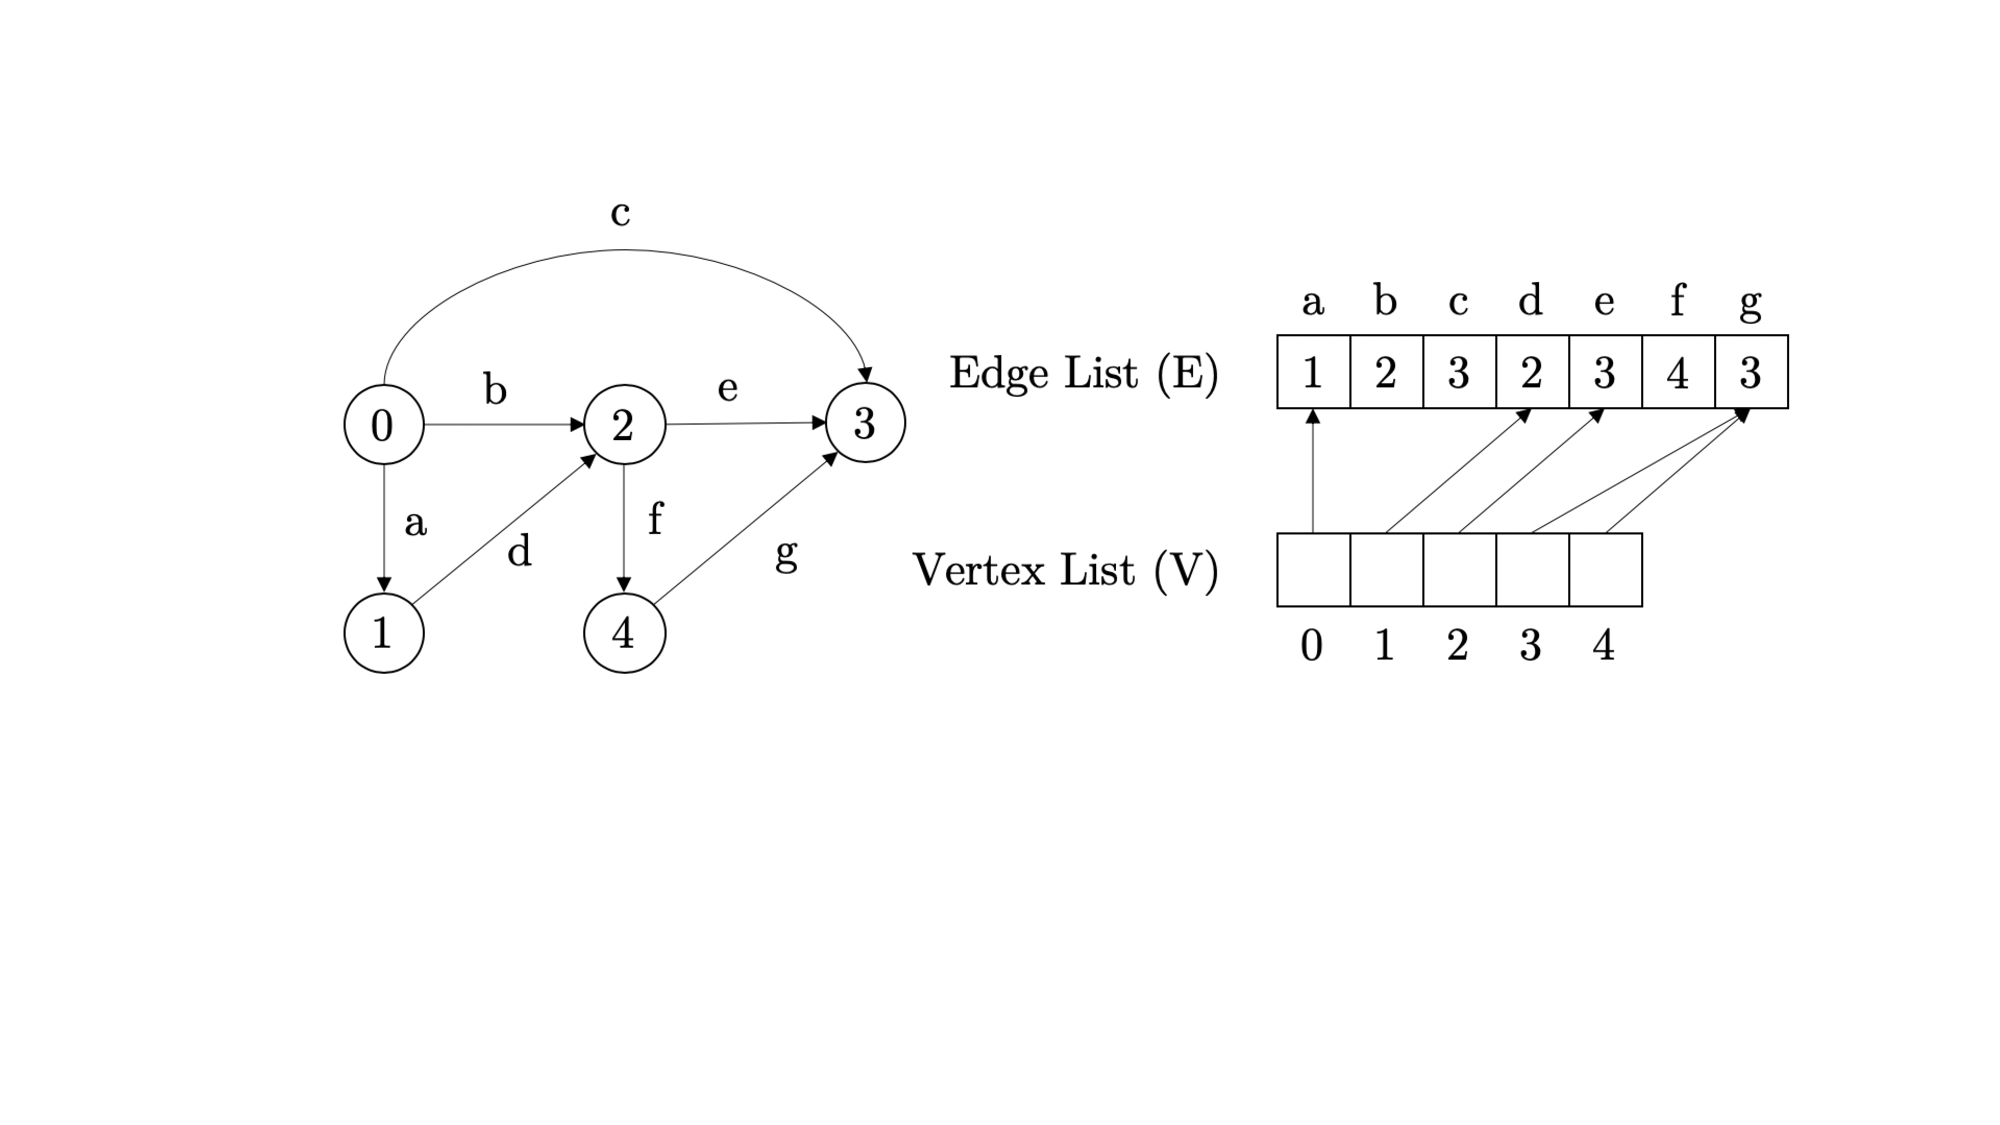
\includegraphics[width=0.8\textwidth]{graphit-figures/graph-format-figure.pdf}
    \caption{The CSR graph format that we use to store graph data on the manycore. For weighted graphs, the weight is stored with each element in the edge array.}
    \label{pap:generals2020:sec:background:fig:graphformat}
\end{figure}
}
\section{GraphIt: A Graph Processing Domain-Specific Language}\label{pap:generals2020:sec:graphit}

GraphIt is a domain-specific language for graph processing applications~\citep{zhang2018graphit}.
Like Halide~\citep{ragan2013halide}, GraphIt separates the description of the algorithm from the scheduling of the computation. A separate algorithm language and scheduling language are used to specify graph programs in GraphIt. This separation of description and schedule allows users to express computation more flexibly.
Listing~\ref{pap:generals2020:sec:background:lst:graphit} shows an example GraphIt program implementing Breadth-First Search (BFS).

\begin{lstlisting}[language=graphit, 
                   caption=GraphIt code for Breadth-First Search (BFS),
                   label=pap:generals2020:sec:background:lst:graphit]
const edges : edgeset{Edge}(Vertex,Vertex);
var frontier : vertexset{Vertex} = new vertexset{Vertex}(0);
const parent : vector{Vertex}(int) = -1;

func updateEdge(src : Vertex, dst : Vertex)
    parent[dst] = src;
end

func toFilter(v : Vertex) -> output : bool
    output =  parent[v] == -1;
end

func main()
    // frontier setup
    while (frontier.getVertexSetSize() != 0)
      #s1# frontier = edges.from(frontier).to(toFilter).applyModified(updateEdge,parent,true);
    end
end

schedule:
  program->configApplyDirection("s1", "DensePull")->generateManycoreCode();
\end{lstlisting}

\subsection{Graph Representation}
Graphs are represented by \lstinline[language=graphit]{edgeset} and \lstinline[language=graphit]{vertexset} structures.
The edges between nodes are stored as an \lstinline[language=graphit]{edgeset}, and any vertex specific data is stored as a \lstinline[language=graphit]{vertexset}.
Line~1 and Line~2 of Listing~\ref{pap:generals2020:sec:background:lst:graphit} demonstrate the declaration of the \lstinline[language=graphit]{edgeset} variable \lstinline[language=graphit]{edges} and  \lstinline[language=graphit]{vertexset} variable \lstinline[language=graphit]{frontier}. 
Any data associated with elements in an \lstinline[language=graphit]{edgeset} or \lstinline[language=graphit]{vertexset} is stored as a \lstinline[language=graphit]{vector}.
Line~3 of Listing~\ref{pap:generals2020:sec:background:lst:graphit} shows the declaration of a \lstinline[language=graphit]{vector} variable, \lstinline[language=graphit]{parent}, that contains data associated with the vertices in the graph.

GraphIt uses Compressed Sparse Row (CSR) graph format for these data structures, illustrated in Figure~\ref{pap:generals2020:sec:background:fig:graphformat}.
CSR format represents a graph with two arrays: a vertex list and an edge list.
The edge list contains the destination vertex for each edge in the graph and contains $|E|$ elements where $E$ is the set of edges in the graph.
In the case of a weighted graph, the edge list is stored as an array of tuples, with each element in the array containing the destination vertex id and the weight of the edge.
The vertex list contains $|V|$ elements where $V$ is the set of vertices in the graph. 
Each element in the vertex list is an index into the edge list array.
This index corresponds to the start of the edges for which that vertex is the source vertex.
The number of edges for a vertex $v$, or its degree, is $vertex\_list[v+1] - vertex\_list[v]$.
The generated code operates on these arrays to perform computation.

\graphformatfig


\subsection{Algorithm Representation}
An algorithm in GraphIt is written as operations on \lstinline[language=graphit]{edgeset} and \lstinline[language=graphit]{vertexset} datatypes. 
Graphit provides several operators that perform computation on these types, but the most common are the \lstinline[language=graphit]{filter} operator and \lstinline[language=graphit]{apply} operator.
The \lstinline[language=graphit]{filter} operator takes a function and a set, applies the function to each element in the set, and returns a set of elements where the function returned true.
The \lstinline[language=graphit]{apply} operator takes a function and set as input and applies the function to each element in the set. %, and returns the resulting set of modified elements.
GraphIt also provides other built-in operators like \lstinline[language=graphit]{applyModified}, that takes a function and a set, applies the function to each element in the set, and returns a vertexset that contains vertices that were updated by the input function. 
This operator is used to construct frontiers in iterative graph algorithms. 
Listing~\ref{pap:generals2020:sec:background:lst:graphit} demonstrates how these operators can be used to write BFS.

Line~16 of Listing~\ref{pap:generals2020:sec:background:lst:graphit} demonstrates two uses of the \lstinline[language=graphit]{filter} operator and one use of the \lstinline[language=graphit]{applyModified} operator. 
The first filter application (\lstinline[language=graphit]{from(frontier)}) selects only edges with source vertices that are in the current frontier. 
The second filter application (\lstinline[language=graphit]{to(toFilter)}) uses the \lstinline[language=graphit]{toFilter} function, defined on line~9, to select edges with destination vertices that haven't been previously visited.
Next, an \lstinline[language=graphit]{applyModified} operator is applied to this filtered set of edges.
This operator computes the edge traversal of BFS and returns a vertexset containing the vertices that were updated by the \lstinline[language=graphit]{updateEdge} function defined on line~5.
This \lstinline[language=graphit]{vertexset} becomes the new frontier for the next iteration of the while-loop.
%\todo[inline]{Check all line-number references}

\subsection{Schedule Representation}
GraphIt provides a wide range of scheduling options, i.e., by specifying traversal direction, by specifying the level of parallelism, or by using load balancing techniques for parallel operators.
Labels are used to indicate which operators in the algorithm description the scheduling optimizations should be applied to.
The separation of the algorithm description and schedule allows developers to iterate through different scheduling optimizations and is a key part of GraphIt.
The schedule finishes by generating code for the target device.
The schedule description always follows the algorithm description in GraphIt.

The schedule for BFSs starts with the \lstinline[language=graphit]{schedule} declaration on Line~20 of Listing~\ref{pap:generals2020:sec:background:lst:graphit}. Line~21 specifies that the schedule for label \lstinline[language=graphit]{#s1#} should be "Dense Pull". This schedule is described in Section~\ref{sec:method}
Finally, the schedule specifies that the code generator should generate code for the target device. 

\subsection{Code Generation}
GraphIt's code generator takes an algorithm and schedule and generates device-specific code.
Graphit first parses the algorithm and schedule using the frontend to produce the Intermediate Representation. 
Next, the compiler performs dependency analysis and enforces restrictions on read-write accesses and reduction operators. 
Once the compiler verifies the validity of the algorithm and schedule, the backend generates code for the target device and host (if necessary).
%Section~\ref{sec:method} describes how our back end generates manycore code.

% !TEX root = paper.tex
\newcommand{\nonblockedMethodFigure}{
\begin{figure}[h]
    \centering
    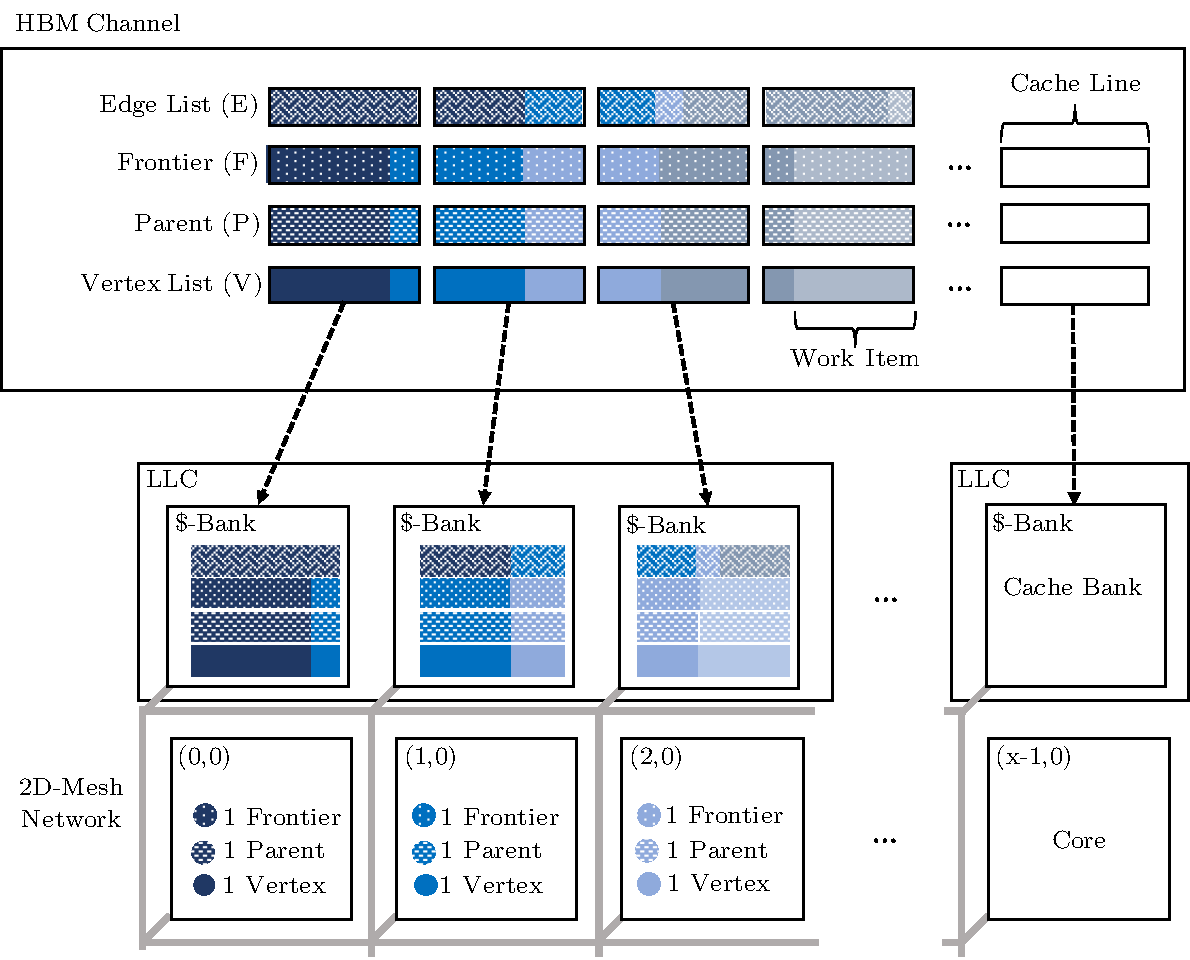
\includegraphics[scale=0.7]{graphit-figures/non-blocked.pdf}
    \caption{Data layout of BFS on the manycore. Data resides in HBM main memory and is cached in LLC. Each core is assigned work items sized without alignment consideration. Cores request single words of data on demand when needed. }
    \label{pap:generals:sec:method:sub:blocked:fig:non-blocked}
\end{figure}
}

\newcommand{\blockedMethodFigure}{
\begin{figure}[t]
    \centering
    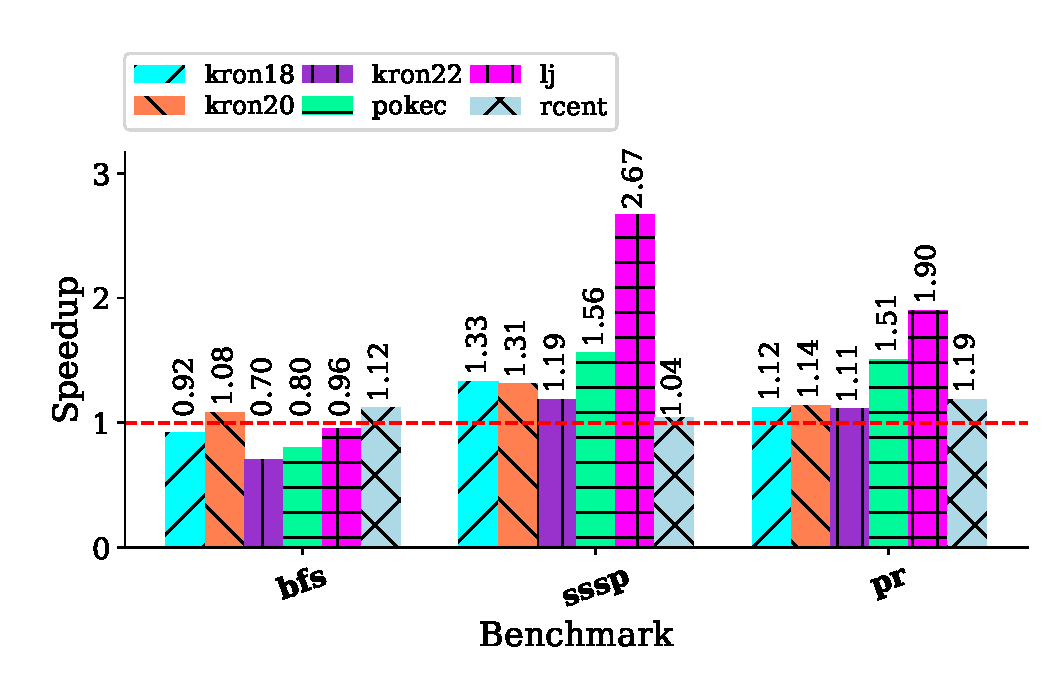
\includegraphics[scale=0.7]{graphit-figures/blocked.pdf}
    \caption{Data layout of BFS with blocked accesses. Cores are assigned cache aligned work items. Cores prefetch entire cache line-sized blocks of data to hide request latency.}
    \label{pap:generals:sec:method:sub:blocked:fig:blocked}
\end{figure}
}

\newcommand{\combinedBlockingFigure}{
\begin{figure*}[t!]
    \centering
    \subfloat[Non-Blocked Accesses]{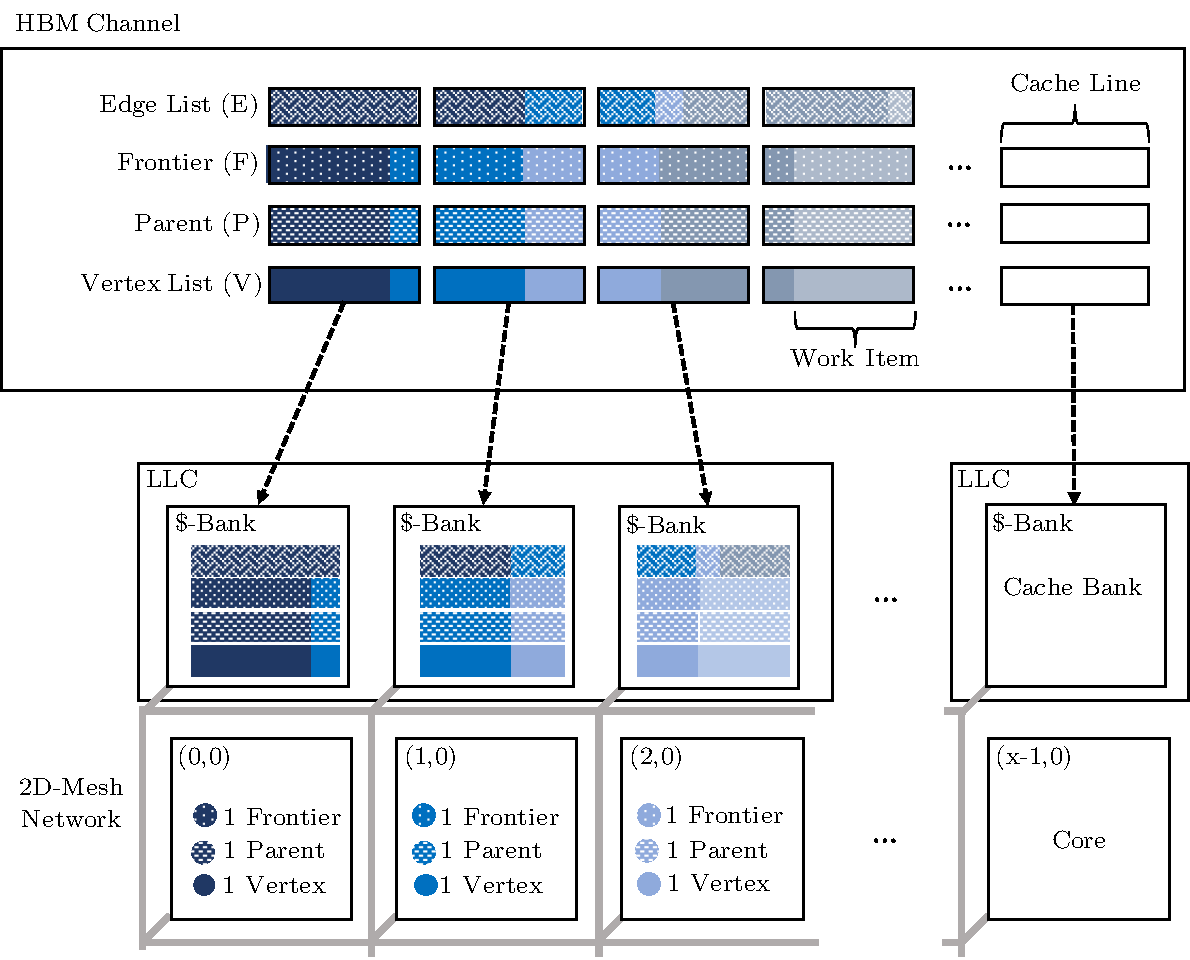
\includegraphics[scale=0.7]{graphit-figures/non-blocked.pdf}}
    \qquad
    \subfloat[Blocked Accesses]{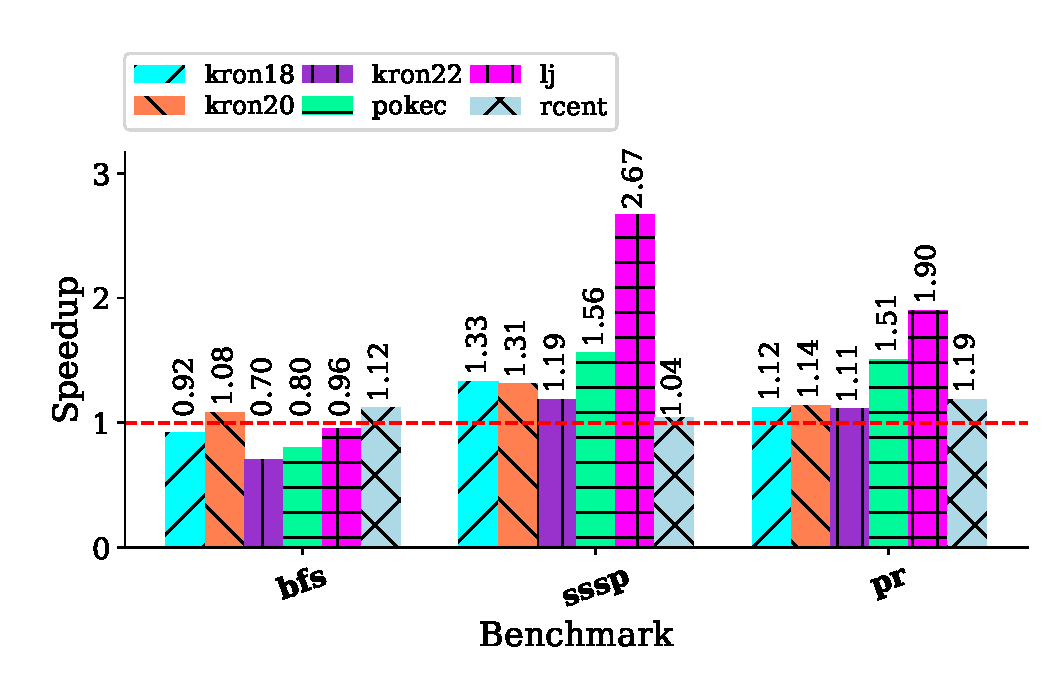
\includegraphics[scale=0.7]{graphit-figures/blocked.pdf}}
    \caption{Data layout of BFS on the manycore. Data resides in HBM main memory and is cached in LLC. In the baseline implementation, each cores are assigned work items sized without alignment consideration and request single words of data on demand when needed. With the blocked access optimization, cores are assigned cache aligned work items and prefetch entire line-sized blocks of data to hide request latency.}
    \label{pap:generals:sec:method:sub:blocked:fig:blocking}
\end{figure*}
}

\newcommand{\edgeAwareMethodFigure}{
\begin{figure}
    \centering
    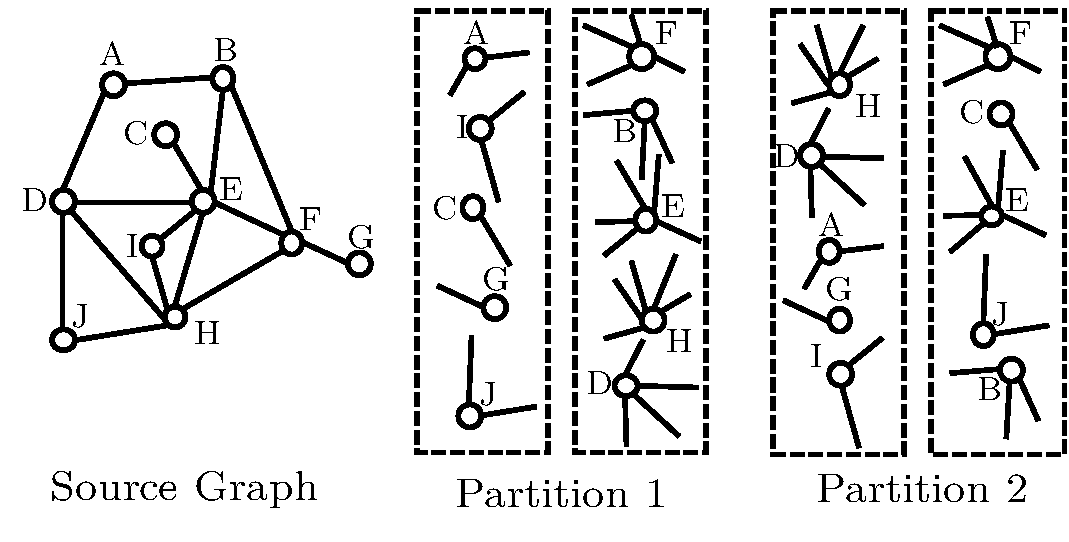
\includegraphics[scale=0.6]{graphit-figures/edge-aware.pdf}
    \caption{Depiction of vertex-based and edge-aware vertex-based partitioning. Partition 1 shows an example vertex-based partitioning between two cores, and Partition 2 shows an example edge-aware partitioning that provides a better workload balance between the two cores.}
    \label{fig:edgeaware}
\end{figure}
}
\newcommand{\edgeAwareMethodAlgorithm}{
\begin{figure}
\centering
\begin{algorithmic}[1]
\Function{Recursive Range}{$start, end$}
\If {$index[end] - index[start] < grain size$}
    \State $core.start \gets start$
    \State $core.end \gets end$
\Else 
    \State $recursive range (start, end/2)$
    \State $recursive range (end/2, start)$
\EndIf
\EndFunction
\end{algorithmic}
\caption{Pseudocode for the recursive call portion of the edge-aware vertex partitioning scheme.}
    \label{alg:edge-aware}
\end{figure}
}
\newcommand{\pushVPullMethodFigure}{
\begin{figure}
    \centering
    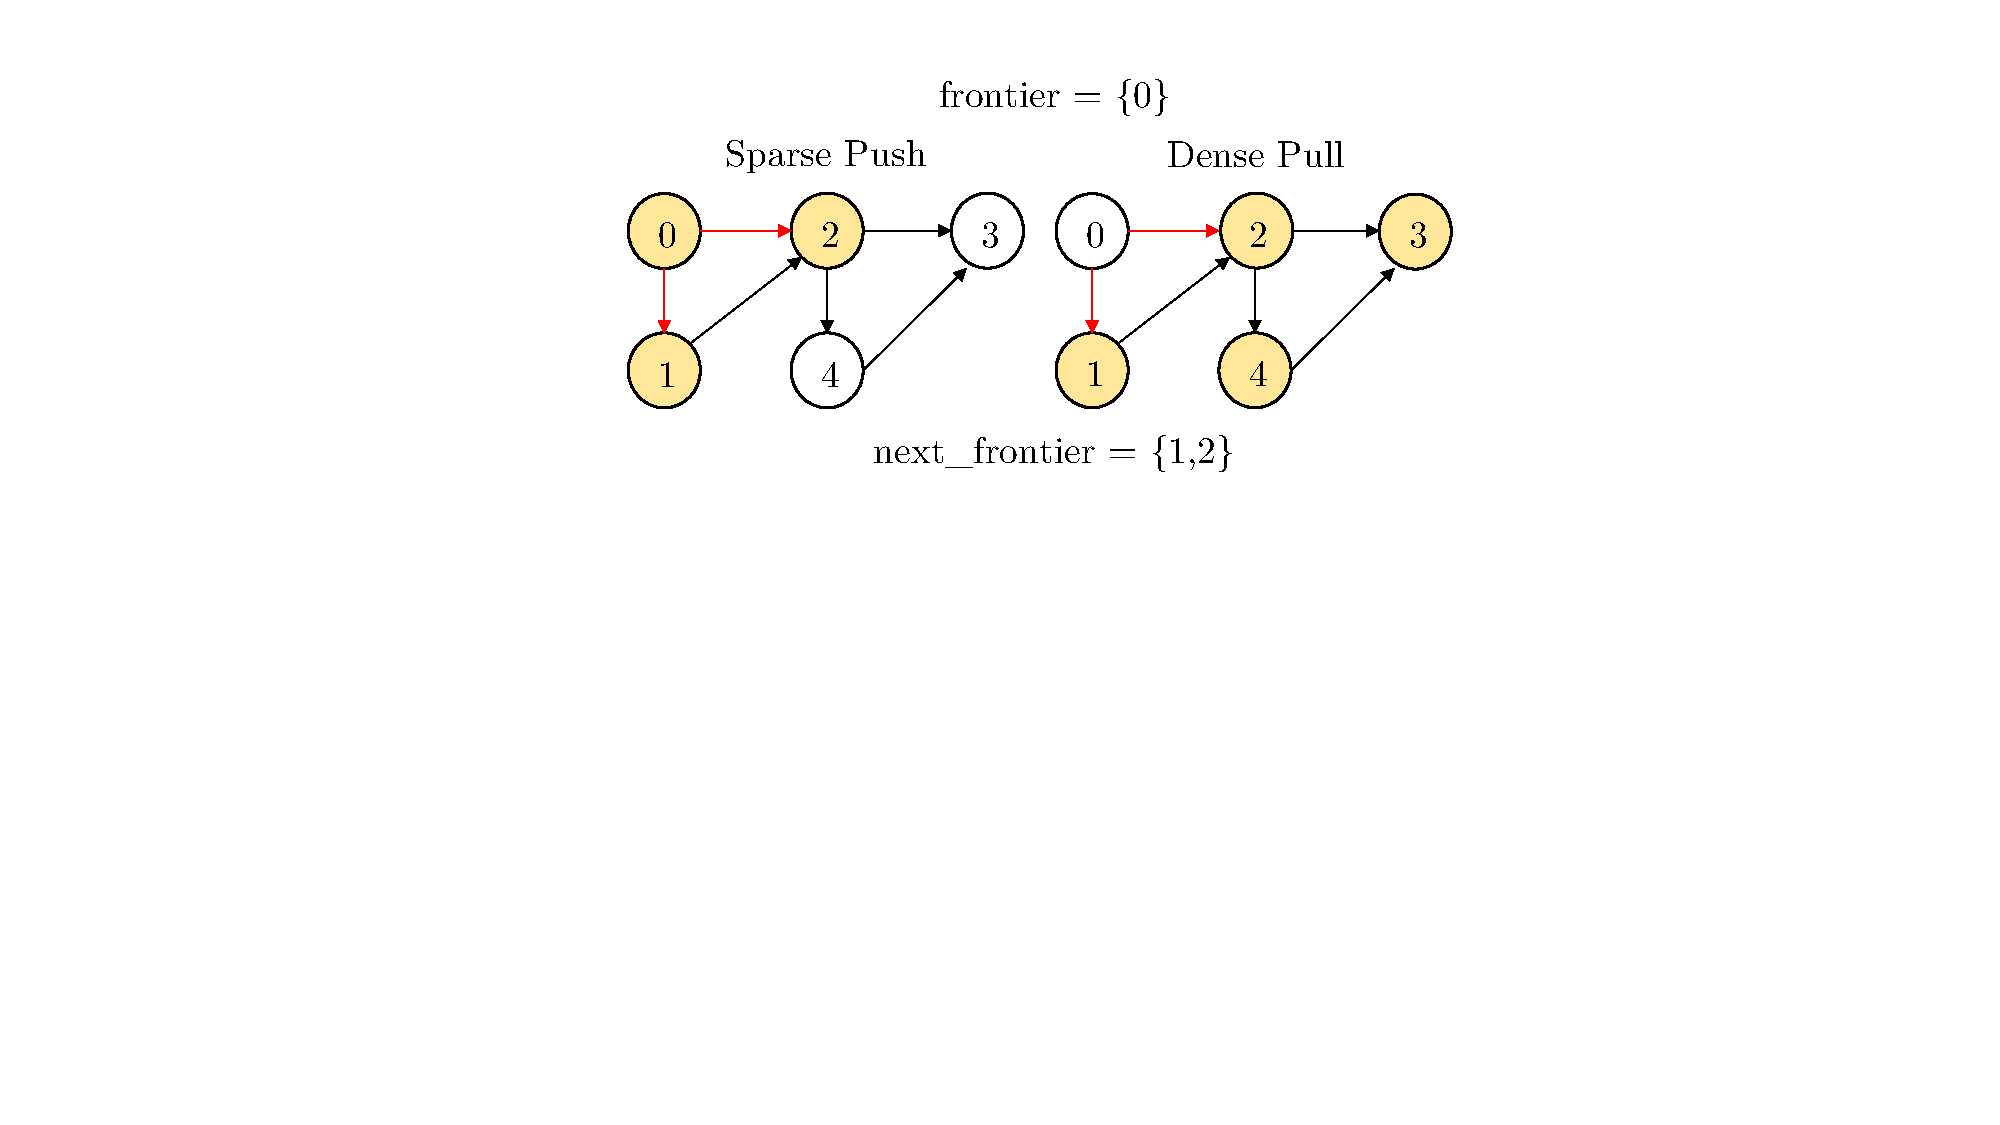
\includegraphics[scale=0.7]{graphit-figures/push_v_pull_fig.pdf}
    \caption{Representation of one iteration of BFS in both the \textsc{Push} and \textsc{Pull} directions. Nodes highlighted in yellow are visited during the iteration. Edges in red are edges that are traversed during execution.}
    \label{fig:pushpull}
\end{figure}
}

\subsection{Performance Optimizations} \label{sec:method}

In this subsection, we explore optimizations to improve graph application performance on the manycore system described in Section \ref{pap:generals:sec:architecture}.
First, we propose a blocked access method for graph data to better exploit memory-level parallelism (MLP) in software.
Next, we discuss three different work partitioning schemes.
%Next, we discuss an implementation of edge-aware vertex partitioning. 
We follow this with an exploration of graph traversal directions.
%Lastly, we introduce a GraphIt backend for a manycore architecture which can automate the process of applying the schedules discussed in this section. 

\subsubsection{Blocked Access Method}\label{sec:method:sub:blocked}
%\combinedBlockingFigure
%Figure \ref{pap:generals:sec:method:sub:blocked:fig:blocking}(a) shows the data layout of BFS on the manycore.
In the naive execution model, cores request single words of application data at the time of use.
The LLC responds to these requests, fetching data from HBM main memory when there is a cache miss.
We discover from profiling that applications spend most cycles waiting on serialized read requests from LLC and DRAM.
Many of these loads occur in iterations of the outer loop between which there are no data dependencies.
%This motivates an optimization in which software reschedules these long-latency memory requests to happen in parallel.
%\nonblockedMethodFigure

\blockedMethodFigure

Software can reschedule these long-latency requests to execute in parallel by formatting work items into blocks.
Cores iterate over their assigned blocks, prefetching the entire block at once.
The block data is stored in the core's scratchpad memory, re-purposing it as a software managed L1 cache.
Figure \ref{pap:generals:sec:method:sub:blocked:fig:blocked} illustrates the blocked memory access technique. 
Work items are stored in HBM in contiguous cache-aligned blocks.
The LLC fetches a block from DRAM after receiving an initial load request from software.
Cores issue these memory requests with an explicit call to \lstinline[language=C++, basicstyle=\small\ttfamily]{memcpy} to exploit pipelined non-blocking loads and hide memory latency.
After fetching the blocked data, cores complete the loaded work before continuing to the next block.
Cores must flush modified blocks back to main memory before fetching the next block.

This blocked access method gives software fine grain control over what data is read at the block and word granularity allowing the application to only prefetch data it is likely to use. 
%For graph applications, this provides benefits when performing random read-modify-writes by increasing the effective memory bandwidth. 
This improves effective cache bandwidth by eliminating false sharing between work items and improves core memory access latency by improving locality for a work item.
%This allows graph applications to take advantage of the spatial locality in the CSR data structure while avoiding over-fetch from performing random updates. 
%For graph applications, this removes over-fetching from random read-modify-writes even as software benefits
%\blockedMethodFigure

% Non-stalling memory operations improves this microarchitecture.
% The \lstinline[language=C++, basicstyle=\small\ttfamily]{memcpy} invoked by software for performing blocked accesses is finely tuned to issue many of these non-stalling loads at once.
% This provides the software with an easy way to exploit the system's MLP.
% Overlapping the time waiting for memory requests to make their way through the network and memory system improve single core performance.

%This blocked memory access optimization has two benefits over a system with hardware managed L1 caches.
%First, it removes the need for hardware to maintain cache coherence, which is hard to scale to a large number of cores \cite{agarwal1988cachecoherence}.
%Second, it gives software finely grained control over what data is read at the block and word granularity.
%As a result, this means applications only need to pay for prefetching data that it is likely to use.
%For graph applications, this blocked memory access method provides benefits when performing random read-modify-writes, as prefetched data in this case is unlikely to be used.

\subsubsection{Work Partitioning} \label{sec:method:sub:edge-aware-partitioning}


We implement and explore the two load balancing methods: vertex-based and edge-aware vertex-based partitioning. We also propose our own manycore specific work partitioning method: alignment-based partitioning. 

\paragraph{Vertex-Based} In vertex-based partitioning, all cores receive an equal number of vertices to traverse. 
In real world graphs, the number of edges per vertex can vary drastically, and due to this, the vertex-based approach can lead to workload imbalance. 

\paragraph{Alignment-Based} 
In alignment-based partitioning, cores work instead on smaller work blocks of vertices that better align with cache lines in the LLC and make better use of the entire memory system by increasing effective bandwidth.
In this method, the vertices in the graph are split into $V/b$ work blocks where $b$ is the number of vertices contained in each work block and $V$ is the total number of vertices in the graph. We select $b$ to be a multiple of the cache line size. By doing this and by reducing the size of the active set of vertices that each core is working on, we are able to increase the cache hit rate and reduce cache line contention.

%This partitioning scheme reduces the size of the active set of vertices that each core is working on at any time.

\paragraph{Edge-Aware Vertex-Based}
\edgeAwareMethodFigure
Edge-aware vertex partitioning scheme considers the number of edges being assigned to each core when partitioning the vertices.
Figure~\ref{fig:edgeaware} demonstrates how edge-aware partitioning differs from vertex-based.

In Figure~\ref{fig:edgeaware}, Partition 1 shows a vertex-based partitioning and Partition 2 represents an edge-aware partitioning of the graph.
In both cases, the number of vertices assigned to each core is 5, but in the vertex-based partitioning scheme the first core is assigned 8 edges and the second core is assigned 21 edges.
This could lead to a large workload imbalance.
In the edge-aware partition, the first core is assigned 14 edges and the second core is assigned 15.
By considering the number of edges being assigned to each core, edge-aware partitioning is able to create a more balanced workload across cores.


In order to accomplish edge-aware vertex-based partitioning, a maximum number of edges that can be assigned to a core is set before execution. 
Edge-aware partitioning effectively does a binary search for partitions of vertices that do not exceed this maximum number of edges. 
Initially, all vertices are considered in one large partition.
%In the first iteration, the core attempts to assign all of the vertices in the graph to itself. 
If this partition of vertices exceeds the number of edges that can be assigned to a core, it is split in half, and each of those partitions are examined as possible candidates.
This process continues recursively until all vertices have been assigned to a core.

In our implementation, a single core is tasked with performing the recursive assignment of work while the remaining cores wait to receive their work assignment. 
While there is overhead introduced by this partitioning scheme, we expect that a more balanced split of work will improve load balance and memory system performance on graph programs with unbalanced input graphs.
%We refer to this value as the grain size.
%In our implementation, the grain size is set to $(E / N) * 1.5$ where $E$ is the total number of edges in the graph and $N$ is the number of cores in the manycore. 
%We found that a buffer value of $1.5$ was necessary to ensure that all of the vertices were assigned across the cores for all sizes of $E$ and $N$ that we examined.

%\edgeAwareMethodAlgorithm


%Figure \ref{alg:edge-aware} shows the pseudocode for this assignment routine.
%In the first iteration, the core attempts to assign all of the vertices in the graph to itself.
%If the number of edges is greater than the grain size, the recursive call is made.
%In the recursive call, the number of vertices in the range is split in half and the core checks if either the first half of the vertices or the second half of the vertices can be assigned to any core. 
%If either of them contain too many edges, the recursive call is made again.


\subsubsection{Graph Traversal Directions}

\pushVPullMethodFigure

In traditional Breadth-First Search, the graph is traversed in a top-down manner by examining the outgoing edges of vertices in the frontier.
For each vertex in the frontier, its edges are traversed and previously unvisited destination vertices are added to the next frontier.
As the size of the frontier grows, the number of edges that need to be traversed also increases.

Beamer et al.~\cite{beamer-bfs-direction} introduced a new method of traversal that reverses the direction in which edges are examined, and showed that this bottom up \pull approach can greatly reduce the number of edges traversed and improve performance. 
In this case, the edges of every vertex in the graph are examined, looking for vertices that are in the current frontier.
There are algorithmic optimizations that can be made in the \pull~direction to reduce the number of vertices and edges that are examined though. 
In BFS for instance, if a node has already been visited in a previous iteration, its edges do not need to be examined in any subsequent iteration.

Figure~\ref{fig:pushpull} shows both the \push~and \pull~directions for one iteration of BFS on a small graph.
In this example, we start the iteration with vertex 0 in the frontier. 
In the \push~case, the outgoing edges of vertex 0 are examined first.
Because vertices 1 and 2 have not been visited before, they are added to the next frontier.
In the \pull~case, all vertices that have not yet been visited are examined.
In this case, the incoming edges of all vertices except vertex 0 are traversed.
If an edge originates at a vertex that is in the current frontier, the destination vertex is added to the next frontier.
In Figure~\ref{fig:pushpull}, vertices 1 and 2 have edges that originate at vertex 0, so they are added to the next frontier. 

Beamer et al.~\cite{beamer-bfs-direction} find that while the \pull~direction increases performance on dense frontiers, traversing the graph in the traditional top down \push direction is still the better option on sparse frontiers and propose a \hybrid~traversal method.
The \hybrid~approach examines the size of the frontier for each iteration in order to determine whether to execute in the \push~or \pull~direction for that iteration.
Our code generator supports generating code in the \pull, \push, and \hybrid~directions.
%In the \push~direction, the graph is traversed first by the vertices in the current frontier.


\subsection{Manycore Code Generation}\label{sec:method:sub:baseline}

Reasoning about these performance optimizations and manycore-specific considerations is a challenging task.
To address this, we developed a code generation backend targeting a manycore architecture.
This code generator alleviates the need for the programmer to have extensive knowledge of the underlying architecture.
%To alleviate the need for the programmer to have knowledge of the underlying manycore architecture, we develop a code generation backend to GraphIt targeting a manycore architecture.

We add support for our backend and the manycore specific optimizations discussed in Section~\ref{sec:method} with minimal changes to the GraphIt frontend scheduling language.
First, we added the option \lstinline[language=graphit]{generateManycoreCode()} which signals to the GraphIt compiler it should generate code for the manycore architecture described in Section~\ref{pap:generals:sec:architecture}.
We also added support for our blocked access method and alignment-based partitioning scheme in the scheduling language. 

In order to generate code that runs on the manycore, we must generate code for both the host CPU and the manycore device.
%An early consideration when designing the backend was how to split the code between host and device. 
We chose to have the host code handle setup and coordination and to have the device code handle the core graph work.
This is a natural split as it allows the manycore to handle the parallel portions of execution and lets the CPU handle the serial portions of work that require an operating system.

\subsubsection{Host Code} 

The host code that we generate handles most of the setup and coordination of the graph program. 
We leverage a set of runtime libraries that we wrote to simplify and generalize the code generation. 
These runtime libraries provide wrappers over our host driver API and handle loading of program data into manycore memory, initializing the manycore and initiating kernel execution on the manycore. 
These runtime libraries provide a level of abstraction which allows for seamless portability of our backend. 
In order to target a different manycore architecture, we would only need to modify these wrapper functions and would not need to modify our code generator.
\newline
\lstset{language=C++,
captionpos=b,
xleftmargin=.05\textwidth,
frame=single,
numbers=left,
framerule=0pt,
aboveskip=1pt,
belowskip=1pt,
framesep=1pt,
basicstyle=\footnotesize\ttfamily,
keywordstyle={[1]\color{darkred}},
keywordstyle={[2]\color{blue}},
keywordstyle={[3]\color{black}\bfseries},
keywordstyle={[4]\color{darkred}\bfseries},
emphstyle=\slshape,
commentstyle=\color{darkgray},
stringstyle=\color{darkgreen}
}
\begin{lstlisting}[language=C++, breaklines=true, 
                   caption=Generated manycore host code for the Breadth-First Search (BFS) program shown in Listing~\ref{pap:generals2020:sec:background:lst:graphit}.,
                   label=pap:generals:sec:method:lst:host]
Graph edges = loadEdgesFromFile(file_path) ;
Vector<int> frontier = new Vector<int>(
        edges.num_nodes(), 0);
Device::Ptr device = Device::GetInstance();
addVertexOnDevice(frontier, root );
while (getVertexSetSizeDevice(frontier) != 0){
      device->enqueueJob("bfs_pull_call",
          {edges.getInIndicesAddr() , 
           edges.getInNeighborsAddr(), 
           frontier.getAddr()}); 
      device->runJobs();
}
\end{lstlisting}
Listing~\ref{pap:generals:sec:method:lst:host} shows a subset of the host code generated for the BFS program shown in Listing~\ref{pap:generals2020:sec:background:lst:graphit} and highlights some of our host side runtime libraries for coordinating placement of data and scheduling of work.

The function \lstinline[language=C++, basicstyle=\small\ttfamily]{loadEdgesFromFile} on line~1 loads a graph from an edgelist, formats the graph into the CSR storage format, and loads it into HBM. 
We also provide functions such as \lstinline[language=C++, basicstyle=\small\ttfamily]{addVertexOnDevice} shown on line~4, which handles the insertion of values into vectors that are stored in HBM. 
Finally, on lines 7 and 11 we have functions for scheduling kernel execution on the manycore: \lstinline[language=C++, basicstyle=\small\ttfamily]{enqueueJob()} and \lstinline[language=C++, basicstyle=\small\ttfamily]{runJobs()}.
The enqueue job function takes the name of a kernel along with a list of parameters for that kernel and schedules it for execution.
Lines~8-10 show the functions we provide to find the address of data structures stored in HBM. 
For vector types, we provide the \lstinline[language=C++, basicstyle=\small\ttfamily]{getAddr()} method.
For graphs, we provide \lstinline[language=C++, basicstyle=\small\ttfamily]{getInIndicesAddr()} and \lstinline[language=C++, basicstyle=\small\ttfamily]{getInNeighborsAddr()} to get the addresses of the index and neighbor arrays respectively.
The \lstinline{runJobs()} function tells the manycore to execute all jobs that have been scheduled through calls to \lstinline[language=C++, basicstyle=\small\ttfamily]{enqueueJob()}.

\subsubsection{Device Code}

All \lstinline[language=graphit]{vertexset} and  \lstinline[language=graphit]{edgeset} operators are generated as device code. Most importantly, this includes apply and filter operations along with the edgeset apply modified operation. 
By default, all of these operators are generated as parallel kernels meant to be executed across the entire manycore. 
To distribute work among cores, we implement a \lstinline[language=C++, basicstyle=\small\ttfamily]{local_range(V, start, end)} library function that takes as input the total number of vertices, a pointer to a start value, and a pointer to an end value.
The function evenly splits the vertices across the cores and sets the start and end values as a contiguous subset of vertices for each core to work on. 
Our backend replaces the call to \lstinline[language=C++, basicstyle=\small\ttfamily]{local_range} with \lstinline[language=C++, basicstyle=\small\ttfamily]{edge_aware_local_range} to do the recursive edge-aware work assignment described in Section \ref{sec:method:sub:edge-aware-partitioning}.
\newline
\begin{lstlisting}[language=C++, breaklines=true, 
                   caption=Generated manycore device code for the Breadth-First Search (BFS) program shown in Listing~\ref{pap:generals2020:sec:background:lst:graphit}.,
                   label=pap:generals:sec:method:lst:device]
template <typename TO_FUNC, typename APPLY_FUNC> int bfs_pull(int *in_indices , int *in_neighbors, int *from_vertexset, TO_FUNC to_func, APPLY_FUNC apply_func) { 
    int start, end;
    local_range(V, &start, &end);
    for ( int d = start; d < end; d++) {
        if (to_func(d)){ 
            for(int s = in_indices[d]; s < in_indices[d+1]; s++) {
                if(from_vertexset[s] == 1) {
                    if(apply_func( in_neighbors[s], d )){ 
                        next[d] = 1; 
                    }
                }
            } //end of loop on in neighbors
        } //end of to filtering
    } //end of outer for loop
    barrier.sync();
    return 0;
}
\end{lstlisting}

Listing~\ref{pap:generals:sec:method:lst:device} shows the main kernel code generated for the inner loop of BFS. 
In this code, we can see the use of the \lstinline[language=C++, basicstyle=\small\ttfamily]{local_range} function on line~3 and the use of a barrier before each core exits the kernel on line~15. 
Lines~4-14 iterate through all of the vertices in the graph, traverse edges that have not yet been visited, and build the next frontier.
The parallelism is achieved by each core executing their own contiguous range of vertices obtained from \lstinline[language=C++, basicstyle=\small\ttfamily]{local_range} at the same time. Once a core is finished with its computation, it waits at the barrier for all other cores to finish before returning the results of the iteration. 

\paragraph{Atomics:}
While atomics can mostly be avoided when traversing in the \pull direction, they are still necessary in some cases and are always necessary during \push traversal.
We leverage lock data structures to implement the necessary atomic operations used in our device code.
We initialize one lock per cache line in the LLCs.
Our profiling showed that this number of locks was sufficient to reduce contention in lock acquisition.
Locks are assigned using a simple hash function on the address of the element for which an atomic operation has been called.


%Figure~\ref{pap:generals:sec:method:sub:blocked:fig:non-blocked} shows how our backend makes use of the memory system on the manycore.
%Cores issue memory requests for single elements of the graph arrays.
%If these elements do not currently reside in cache, a request is issued to the HBM. 
%A cache line worth of data is returned from HBM and the single requested element is forwarded back to the core that issued the request.
%Unsurprisingly, our initial tests showed that our graph programs are bound by memory access latency. 
%The blocking optimization proposed in Section \ref{sec:method:sub:blocked} can be enabled by adding \lstinline[language=graphit]{setApply("s1", "enable_blocking")} to a GraphIt schedule like the one shown on line~21 of Listing~\ref{pap:generals:sec:background:lst:graphit}.


%% !TEX root = thesis.tex
%\newcommand{\baselineEvalFigure}{
\begin{figure}[t]
    \centering
    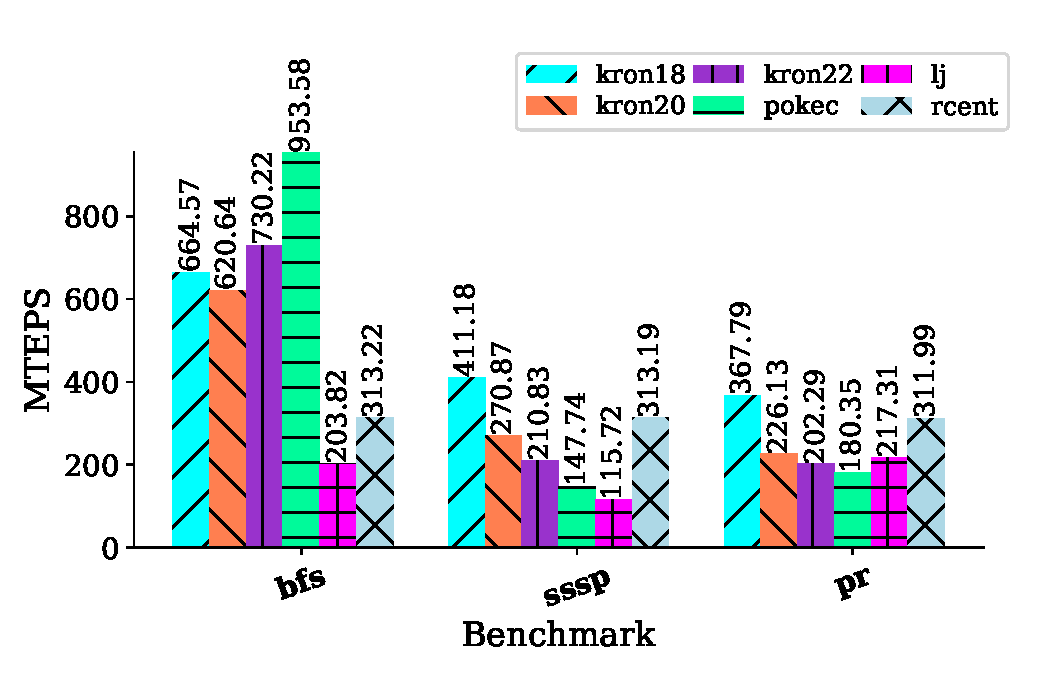
\includegraphics[scale = 0.5]{graphit-figures/baseline.pdf}
    \caption{Baseline code generation results for each benchmark in the dense pull direction with no manycore specific optimizations.}
    \label{pap:generals:sec:eval:fig:baseline}
\end{figure}
}

\newcommand{\pushEvalFigure}{
\begin{figure}[t]
    \centering
    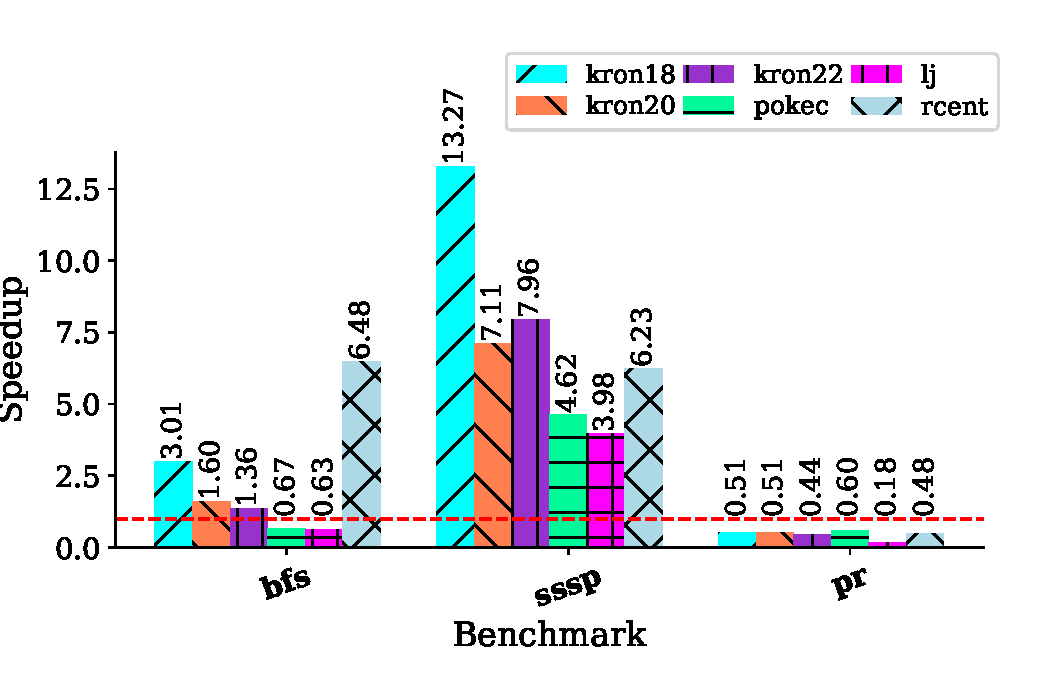
\includegraphics[scale = 0.5]{graphit-figures/push.pdf}
    \caption{Baseline code generation results for each benchmark in the push direction with no manycore specific optimizations.}
    \label{pap:generals:sec:eval:fig:push}
\end{figure}
}

\newcommand{\edgeSpeedupFigure}{
\begin{figure}[t]
    \centering
    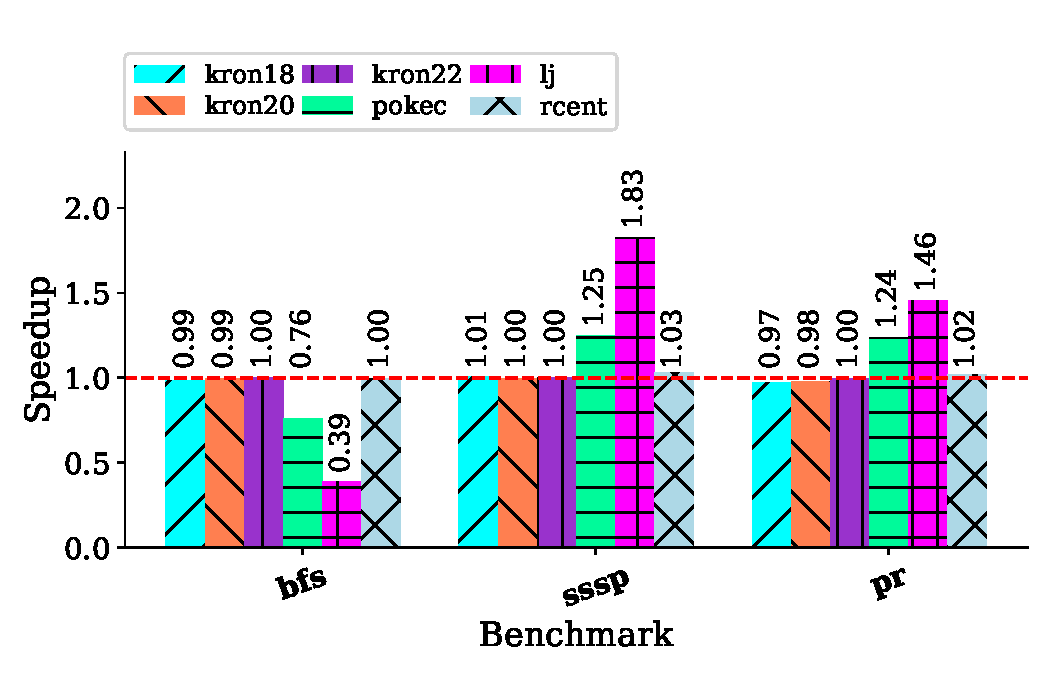
\includegraphics[scale = 0.5]{graphit-figures/edge.pdf}
    \caption{Speedup results for edge based optimization over the baseline dense pull implementation for each benchmark.}
    \label{pap:generals:sec:eval:fig:edge}
    \vspace{-2mm} 
\end{figure}
}

\newcommand{\blockBFSFigure}{
\begin{figure}[t]
    \centering
    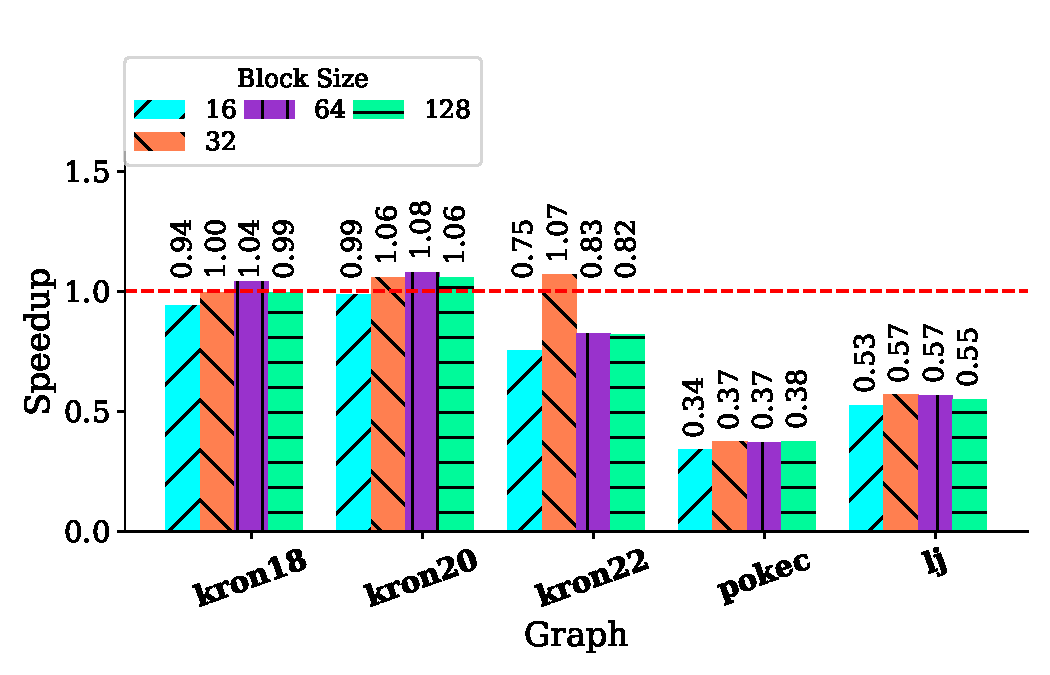
\includegraphics[scale = 0.5]{graphit-figures/bfs-block.pdf}
    \caption{MTEPS results for varying block sizes using the blocked access method on BFS.}
    \label{pap:generals:sec:eval:fig:bfsblock}
\end{figure}
}

\newcommand{\blockSSSPFigure}{
\begin{figure}[t]
    \centering
    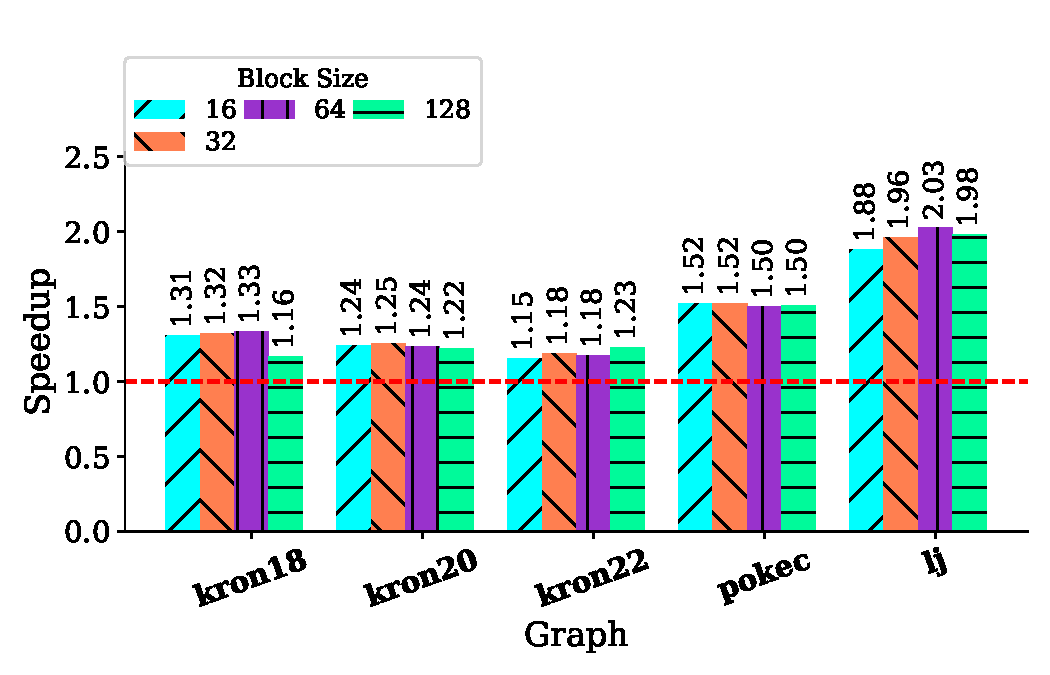
\includegraphics[scale=0.5]{graphit-figures/sssp-block.pdf}
    \caption{Speedup results for varying block sizes using the blocked access method on SSSP. Speedup is calculated over the baseline pull direction implementation.}
    \label{pap:generals:sec:eval:fig:ssspblock}
\end{figure}
}

\newcommand{\cacheBFSFigure}{
\begin{figure}[t]
    \centering
    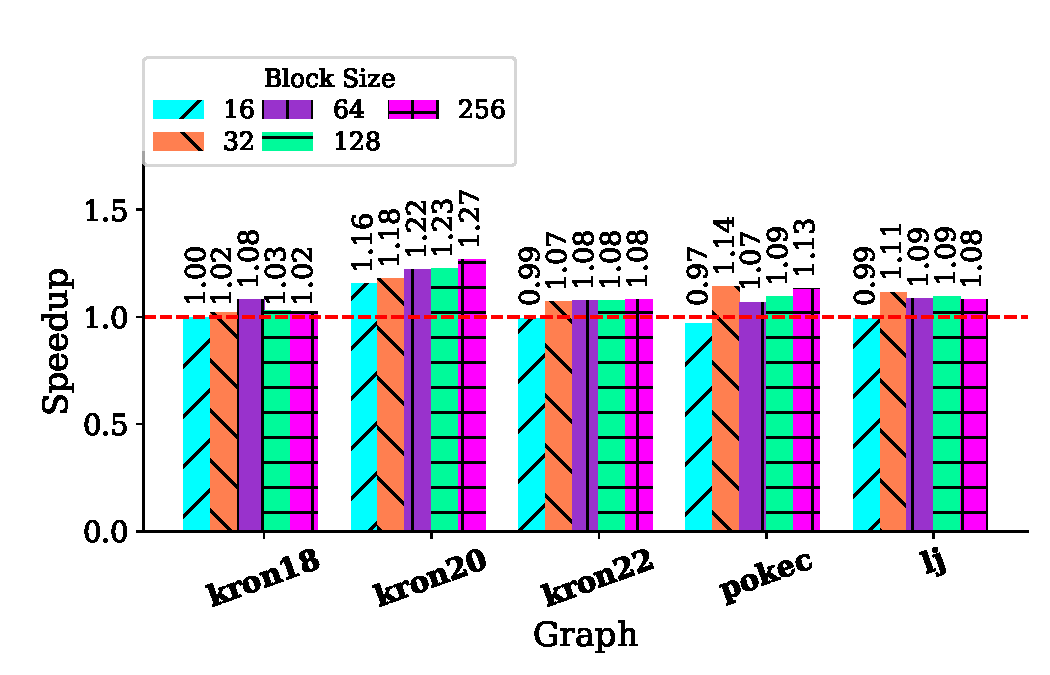
\includegraphics[scale = 0.5]{graphit-figures/bfs-cache.pdf}
    \caption{MTEPS results for varying work block sizes using the manycore aware vertex partitioning scheme on BFS.}
    \label{pap:generals:sec:eval:fig:bfscache}
\end{figure}
}

\newcommand{\cacheSSSPFigure}{
\begin{figure}[t]
    \centering
    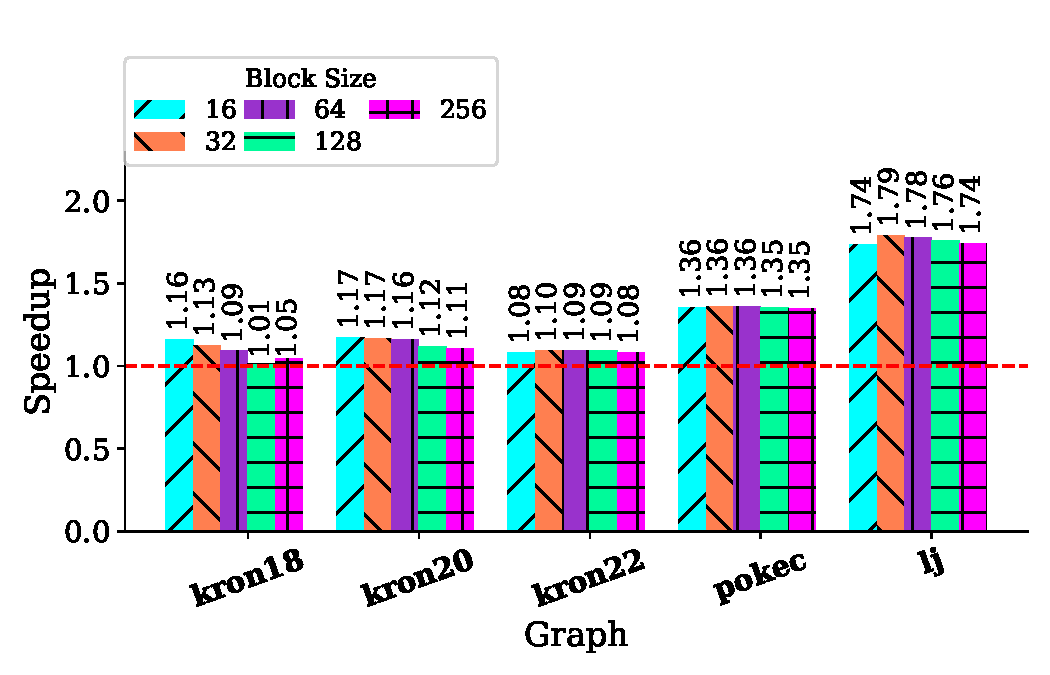
\includegraphics[scale=0.5]{graphit-figures/sssp-cache.pdf}
    \caption{Speedup results for varying work block sizes using the manycore aware vertex partitioning scheme on SSSP. Speedup is calculated over the baseline pull direction implementation.}
    \label{pap:generals:sec:eval:fig:ssspcache}
\end{figure}
}

\newcommand{\allBlockedFigure}{
\begin{figure}[t]
    \centering
    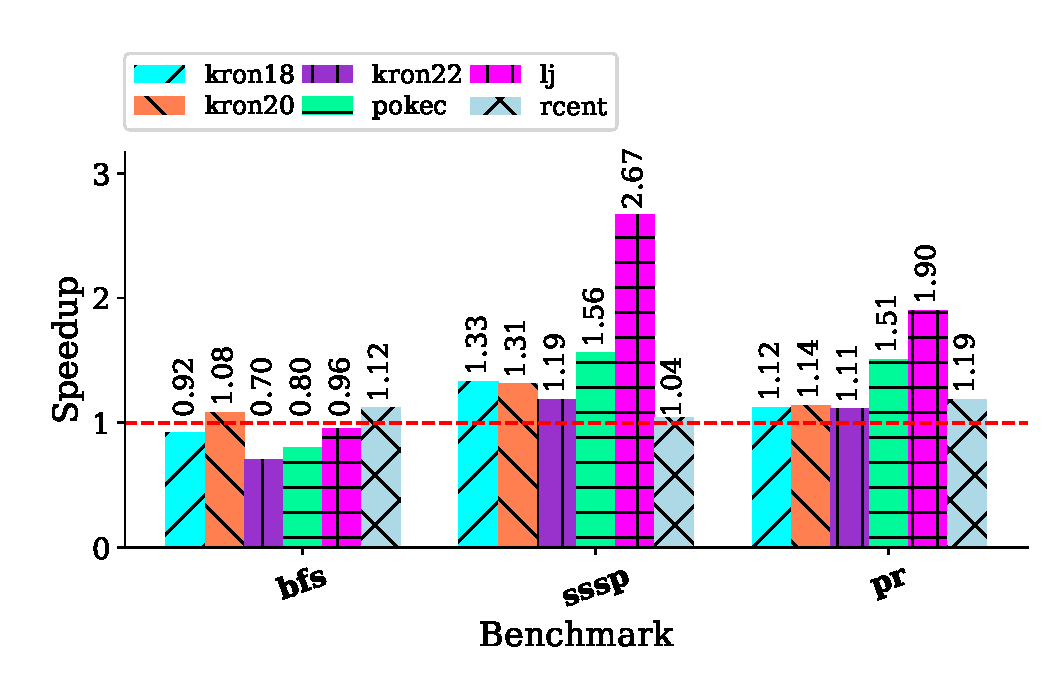
\includegraphics[scale = 0.5]{graphit-figures/all-blocked.pdf}
    \caption{Blocked access method speedup results for each benchmark. Speedup is calculated over the baseline pull direction implementation.} %For each graph and benchmark, block sizes of 16, 32, 64, and 128 elements were tested and the best performing block size is reported here.
    \label{pap:generals:sec:eval:fig:blocked}
\end{figure}
}

\newcommand{\allAlignedFigure}{
\begin{figure}[t]
    \centering
    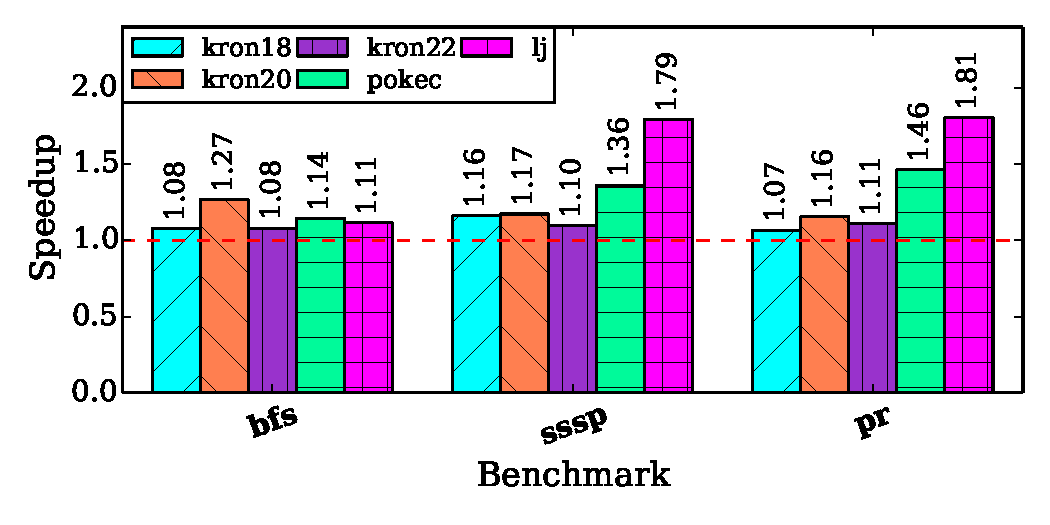
\includegraphics[scale = 0.5]{graphit-figures/align.pdf}
    \caption{Alignment-based partitioning speedup results for each benchmark. Speedup is calculated over the baseline pull direction implementation.} %For each graph and benchmark, work group sizes of 16, 32, 64, 128, and 256 vertices were tested and the best performing work group size is reported here.
    \label{pap:generals:sec:eval:fig:aligned}
    \vspace{-2mm} 
\end{figure}
}

%I am not sure if this is the best way to present an overview of results or if we need it. 
\newcommand{\overviewResultsTable}{
\begin{table}[]
\centering
\begin{tabular}{lrcl}
%\hline
\toprule
\textbf{Benchmark} & \textbf{Graph} & \textbf{MTEPS} & \textbf{Optimization} \\ \midrule
 \multirow{5}{*}{BFS}& kron18 & 457.09 & Cache-Aligned \pull \\ %\cline{2-4}
 & kron20 & 296.32 & Cache-Aligned \pull \\ %cline{2-4}
 & kron22 & 241.95 & Cache-Aligned \pull \\ %\cline{2-4}
 & pokec & 148.02 &  Cache-Aligned \pull\\ %\cline{2-4}
 & lj & 304.36 & Cache-Aligned \pull \\ \hline
 \multirow{5}{*}{PR}& kron18 & 412.34 & Blocked \pull \\ %\cline{2-4}
 & kron20 & 261.35 & Cache-Aligned \pull \\ %\cline{2-4}
 & kron22 & 224.88 & Blocked \pull \\ %\cline{2-4}
 & pokec & 272.57 & Blocked \pull \\ %\cline{2-4}
 & lj & 413.06 & Blocked \pull \\ \hline
 \multirow{5}{*}{SSSP}& kron18 & 467.08 & Cache-Aligned \pull \\ %\cline{2-4}
 & kron20 & 364.36& Baseline \push \\ %\cline{2-4}
 & kron22 & 404.27 & Baseline \push \\ %\cline{2-4}
 & pokec & 149.17 & Cache-Aligned \pull \\ %\cline{2-4}
 & lj & 268.87 & Cache-Aligned \pull \\ %\hline
 \bottomrule
\end{tabular}
\caption{Table containing best MTEPS results across all benchmarks and input graphs. The optimizations used to achieve these results are also listed above.}
\label{pap:generals:sec:eval:tab:overview}
\end{table}
}

\newcommand{\relatedMTEPSTable}{
\begin{table}[]
\centering
\begin{tabular}{cllll}
%\hline
\toprule
 \textbf{Source} & \textbf{Platform} & \textbf{Benchmark} & \textbf{Graph}  & \textbf{MTEPS} \\ \midrule
 \cite{slota2015high}& Xeon Phi MIC & CC & LJ (22) & 240 \\ %\hline
 \cite{slota2015high}& Xeon Phi MIC & CC & Flickr (19) & 140\\ %\hline
 %Galois \cite{aasawat2018well}& Ivy Bridge & PR & LJ (22) & 207.67 \\ \hline
 \cite{khorasani2014cusha} & GTX780 & BFS & LJ (22) & 272.4 \\ %\hline
 \cite{zhong2013medusa}& C2050 & BFS & KKT (21) & 351.5 \\ %\hline
 \cite{yang2019graphblast}& k40c & SSSP & LJ (22) & 334.2 \\ %\hline
 \cite{wang2016gunrock} & k40c & SSSP & LJ (22) & 217.9 \\
 \bottomrule

\end{tabular}
\caption{Performance results in MTEPS from other graph processing frameworks. The benchmark CC is strongly connected components.}
\label{sec:related:tab:mteps}
\vspace{-1mm} 
\end{table}
}
\newcommand{\graphInfoTable}{
\begin{table}[]
\centering
\begin{tabular}{c|c|c|c}
%\hline
 \textbf{Name} & \textbf{Scale} & \textbf{\# Vertices} & \textbf{\# Edges} \\ \hline %\hline
 kron18 & 18 & 262,144 & 4,194,304 \\ \hline
 kron20 & 20 & 1,048,576 & 16,777,216 \\ \hline
 kron22 & 22 & 4,194,304 & 67,108,864 \\ \hline
 pokec & 20.5 & 1,632,803 & 30,622,564 \\ \hline
 livejournal (lj) & 22 & 3,997,962 & 34,681,189 \\ %\hline
\end{tabular}

\caption{The vertex and edge information for each of the graphs used in our evaluation. We use synthetic \kron graphs used in the Graph500 benchmark and two real world graphs.}
\label{sec:eval:tab:graphs}
\end{table}
}

%\subsection{Evaluation} \label{sec:eval}
%In this subsection, we evaluate the performance of our GraphIt code generation backend and its optimizations outlined in Sections~\ref{sec:method} and~\ref{sec:method:sub:baseline}.
%We compare the performance of our generated code to a CPU baseline and evaluate the performance of each of the optimizations we outlined in Section~\ref{sec:method}. 

\section{Experimental Setup}

%\graphInfoTable
\begin{table}[]
    \centering
    \begin{tabular}{c|c|c|c}
    %\hline
     \textbf{Name} & \textbf{Scale} & \textbf{\# Vertices} & \textbf{\# Edges} \\ \hline %\hline
     kron18 & 18 & 262,144 & 4,194,304 \\ \hline
     kron20 & 20 & 1,048,576 & 16,777,216 \\ \hline
     kron22 & 22 & 4,194,304 & 67,108,864 \\ \hline
     pokec & 20.5 & 1,632,803 & 30,622,564 \\ \hline
     livejournal (lj) & 22 & 3,997,962 & 34,681,189 \\ %\hline
    \end{tabular}
    
    \caption{The vertex and edge information for each of the graphs used in our evaluation. We use synthetic \kron graphs used in the Graph500 benchmark and two real world graphs.}
    \label{sec:eval:tab:graphs}
\end{table}

Host software executes natively on an Intel Xeon Gold 6254 CPU.
The host libraries interface directly with the simulator environment using the SystemVerilog DPI interface.
We compile all generated C++ code using the GNU Compiler Collection (GCC) with ``-O2''.

\paragraph{Manycore Architecture}
% We evaluate our compiler using detailed RTL simulation of our manycore architecture.
We model a manycore system running at 1GHz with 16 columns and 8 rows for a total of 128 cores.
The machine has a 512KB 8-way set associative LLC with 128-byte lines.
The memory system uses two HBM2 memory channels.
We model the HBM2 memory system with DRAMSim3\cite{li2019dramsim3},  a timing accurate simulator for modeling DRAM.
We use detailed, cycle-accurate RTL simulation to model our processor cores, network on chip, and LLC.
Our simulation environment includes SystemVerilog bind modules for collecting performance metrics such as instruction and cycle counts.
The RTL for this manycore has been validated in silicon, and this configuration occupies approximately 3.5 mm$^2$ of die area. 
%We also collect other profiling statistics such as processor stalls and opcode histograms.

\paragraph{Benchmarks} We evaluate our compiler on three common graph benchmarks: Breadth-First Search (BFS), Single Source Shortest Path (SSSP), and PageRank (PR). 
BFS has a high memory access to computation ratio and is a component of many graph algorithms.
PageRank computes the importance of each vertex in the graph, and unlike BFS, spends most of its time performing computation on the entire graph.
PR also users floating point operations.
%SSSP operates on a weighted graph.
SSSP operates on a larger subset of the edges during execution and tends to be more sensitive to load balancing.
We implement the Bellman-Ford variant of SSSP for our evaluation.

We implement all of these benchmarks in GraphIt and generate manycore code using our GraphIt code generation backend.
Due to the time costs of simulation, we do not run all iterations of our benchmarks. 
For BFS and SSSP, we run one iteration from the middle of execution with a maximal root node selected as the initial frontier.
For PR, we run one iteration from the beginning of execution.



\paragraph{Graphs} We use two types of graphs in our evaluation: synthetic \kron graphs used in the Graph500 benchmark~\cite{murphy2010graph500} and real-world, social network graphs.
\kron graphs follow a power law distribution in order to simulate the small world property often seen in real world graphs~\cite{leskovec2010kronecker}.
We generate three \kron graphs of varying size. 
%We generate weighted and unweighted versions of each of these graphs for use with our three benchmarks.
We use two real-world graphs: pokec~\cite{pokec} and livejournal~\cite{lj}.
All of the graphs we use and their properties are shown in Table~\ref{sec:eval:tab:graphs}.


\section{Results}
%\baselineEvalFigure
\begin{figure}[t]
    \centering
    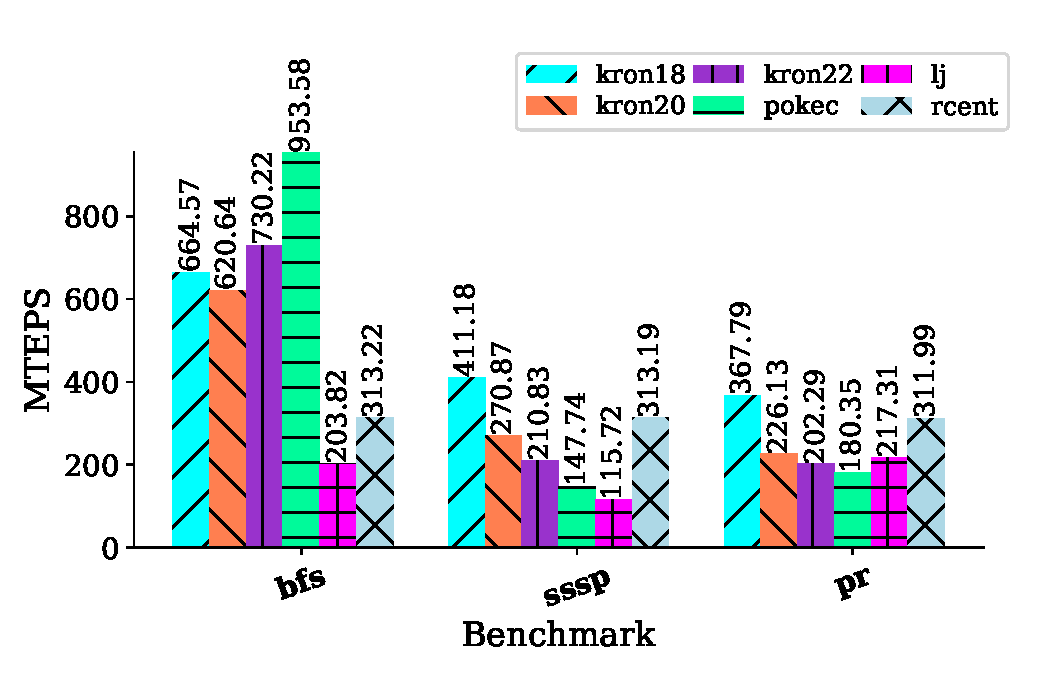
\includegraphics[scale = 0.5]{graphit-figures/baseline.pdf}
    \caption{Baseline code generation results for each benchmark in the dense pull direction with no manycore specific optimizations.}
    \label{pap:generals:sec:eval:fig:baseline}
\end{figure}

%\todo[inline]{Results intro}
To evaluate our code generator, we first present performance results for the unoptimized benchmarks. 
We then explore the performance trade-offs and benefits for each of the optimizations described in Section~\ref{sec:method}.

\subsection{Baseline}
 
%\pushEvalFigure
\begin{figure}[t]
    \centering
    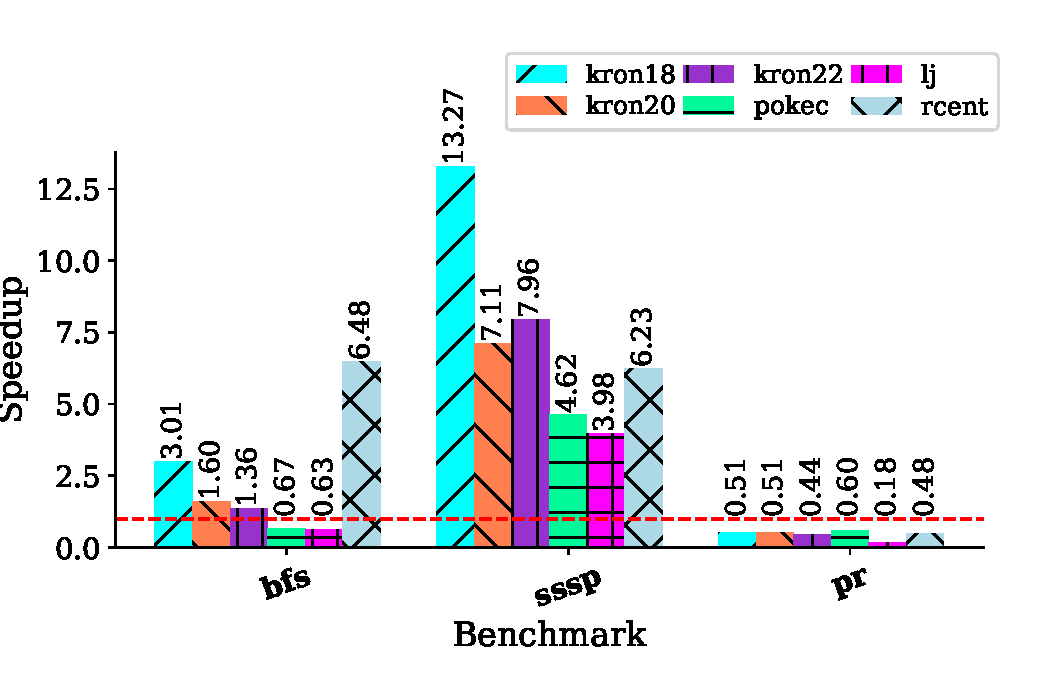
\includegraphics[scale = 0.5]{graphit-figures/push.pdf}
    \caption{Baseline code generation results for each benchmark in the push direction with no manycore specific optimizations.}
    \label{pap:generals:sec:eval:fig:push}
\end{figure}
To establish a baseline, we examine the performance of the code produced by our backend without any added optimizations.
To evaluate performance, we calculate the traversed edges per second (TEPS) for each iteration of each benchmark using the cycle counts that we obtain from simulation.

Figures~\ref{pap:generals:sec:eval:fig:baseline} and~\ref{pap:generals:sec:eval:fig:push} show our initial performance results for the manycore code generated by our backend without added optimizations in the \pull~and \push~directions respectively as described in Section~\ref{sec:method:sub:baseline}.
Across all of these, we see a geometric mean of 214 MTEPS in the \pull~direction and 104 MTEPS in the \push~direction. 
This decrease in performance in the \push~direction is expected as the iterations we examine for BFS and SSSP have very dense frontiers that benefit from traversing in the \pull~direction.
In all three benchmarks, we see the highest performance on the \kron scale 18 graph.
This is most likely due to the relative small size of the graph and the large amount of parallelism and memory bandwidth present on the manycore architecture.
 
BFS has a very high memory access to compute ratio, so the number of reads greatly affects the performance.
Because we use iterations from the middle of execution, a large number of vertices do not need to be visited in the \pull~direction that would need to be visited in the \push~direction. %because they have already been visited in previous iterations.
We see an average increase in performance of 3.6$\times$ just from traversing in the \pull~direction instead of \push. 
 
We see less clear results with SSSP.
For SSSP we observe better performance in the \pull~direction on the real world graphs, but not on the two larger \kron graphs.
From our simulation results, we are able to see that these \kron graphs make better use of the LLCs and issue fewer reads to HBM in the \push~direction, accounting for the improvement in performance. 
 
Interestingly, PageRank sees a performance improvement across all graphs in the \pull~direction.
Unlike BFS, PageRank must visit all vertices in all iterations regardless of traversal direction.
When we examined our simulation results, we saw that the \pull~direction issued fewer read requests to HBM which most likely accounts for the difference in performance. 
 
% \cpuResultsTable
  
% To contextualize these results, we include parallel CPU results in MTEPS for each benchmark and input graph in Table~\ref{pap:cgp21:sec:eval:tab:cpuresults}.
% We generate the parallel C++ code for these tests using the GraphIt CPU backend and run with OpenMP.
% We run these tests on a 4 socket, 72 core, 144 hyperthread, Intel Xeon Gold 6254 CPU running at 3.10 GHz with 25 MB LLC and 3 TB of DDR4 running at 2666MHz.
% It is challenging to provide a direct performance comparison between the two architectures because they are optimized for different goals.
% The Xeon is a high-performance server class CPU with relatively high area and power budgets.
% By contrast, the manycore is designed to be a flexible and low-cost substrate for parallel compute.
%\todo[inline]{somehow expand here and explain why we don't do more of a comparison. maybe also mention that we are simulating only a portion of the entire manycore}
% Manycore is optimized for area and power vs the Xeon optimized for performance.
% We are simulating a quarter of a real chip due to the constraints of our detailed simulation infrastructure.
%The Xeon is a server class CPU with a latency-optimized memory system and relatively high area and power budgets.
%The manycore uses only a tiny fraction of the die area of a Xeon and is designed to achieve best performance per Watt.
 
\subsection{Blocking}
%\blockSSSPFigure
\begin{figure}[t]
    \centering
    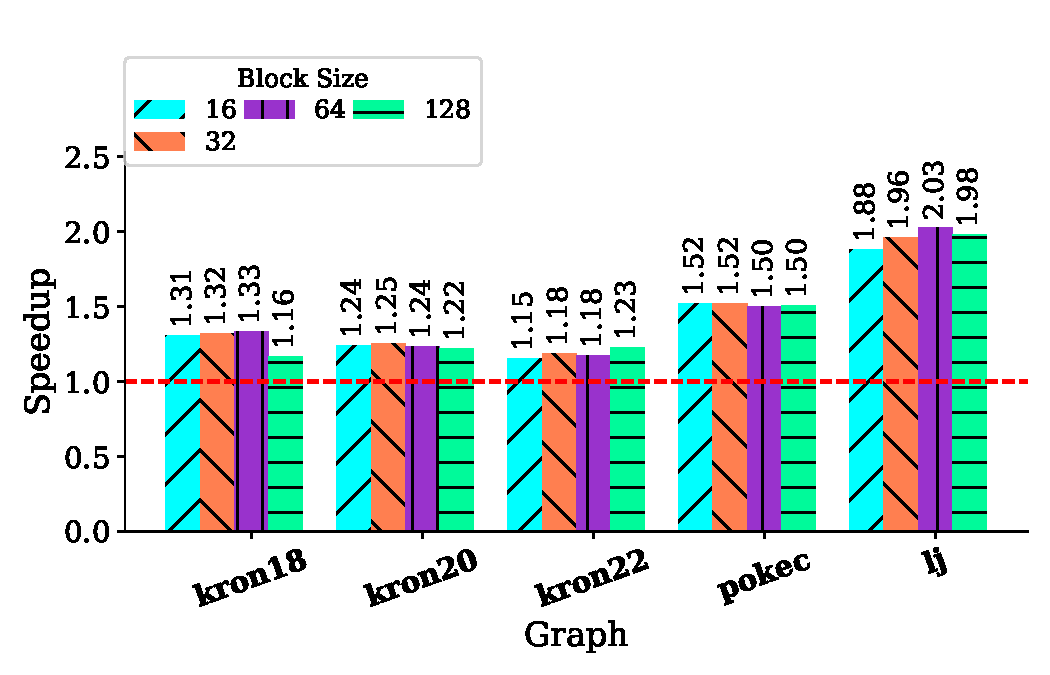
\includegraphics[scale=0.5]{graphit-figures/sssp-block.pdf}
    \caption{Speedup results for varying block sizes using the blocked access method on SSSP. Speedup is calculated over the baseline pull direction implementation.}
    \label{pap:generals:sec:eval:fig:ssspblock}
\end{figure}
 
%\allBlockedFigure
\begin{figure}[t]
    \centering
    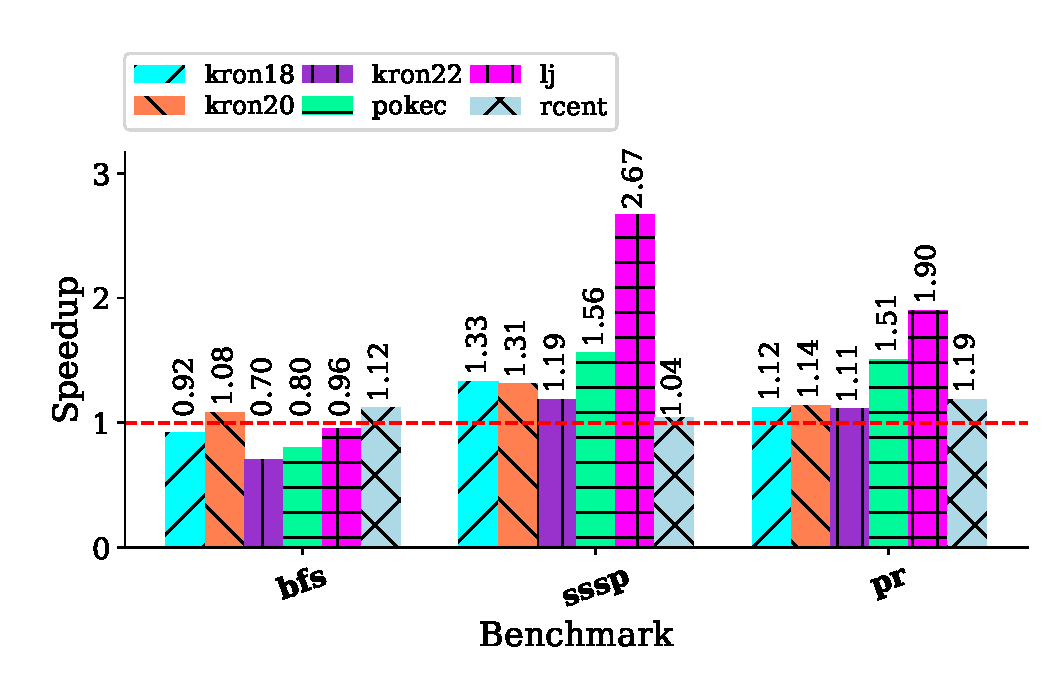
\includegraphics[scale = 0.5]{graphit-figures/all-blocked.pdf}
    \caption{Blocked access method speedup results for each benchmark. Speedup is calculated over the baseline pull direction implementation.} %For each graph and benchmark, block sizes of 16, 32, 64, and 128 elements were tested and the best performing block size is reported here.
    \label{pap:generals:sec:eval:fig:blocked}
\end{figure}
 
Figure~\ref{pap:generals:sec:eval:fig:ssspblock} shows the performance benefit of the blocking optimization across different block sizes on the SSSP benchmark in the \pull~direction. Results for block sizes of 16, 32, 64, and 128 elements are shown.
Speedup is normalized to the baseline performance of SSSP in the \pull~direction without any optimizations.
 
Interestingly, we do not see much variation in speedup across different block sizes. 
Livejournal and \kron 18 see the most speedup with a block size of 64, pokec and \kron 20 see optimal performance with block size 32, and a block size of 128 is optimal for \kron 22. 
We observe that the optimal block size appears to be input graph dependent for the other benchmarks we studied as well. 
 
Figure~\ref{pap:generals:sec:eval:fig:blocked} shows the speedup for each benchmark when using the blocked access method. 
Again, speedup is normalized to the baseline performance of each benchmark in the \pull~direction.
In this figure, the optimal block size for each input graph and benchmark is used in computing the speedup. 
Blocking provides a mean speedup of 1.21$\times$ and a maximum speedup of 2.01$\times$. 
 
Blocking is primarily motivated by the microarchitecture's ability to hide memory load latency.
The prefetching effect from blocking can yield significant performance improvement, but it also provides the effect of data caching.
Even if the data is used once, the prefetching effect can yield significant performance improvement. 
We observe the most speedup with SSSP because it traverses more edges than BFS and benefits most from prefetching.
We see the least speedup from blocking with BFS and see performance degredation on the pokec and livejournal graphs.
The \pull~direction for BFS traverses the fewest edges of the three workloads thanks to a filter condition on destination vertices.
This means that much of the prefetched data is never used, and the additional memory reads become overhead.

Overall, we find that our blocking optimization provides performance improvement in all but two cases. 
Blocking reduces stalls from memory system requests and improves the hit rate of the LLC. We find, however, that it does not have a large impact on DRAM stalls.
Making use of the low-latency scratchpad memory and coalescing accesses most improve performance on benchmarks that traverse more edges in the graph. 
 
\subsection{Work Partitioning}
 
%\cacheSSSPFigure
\begin{figure}[t]
    \centering
    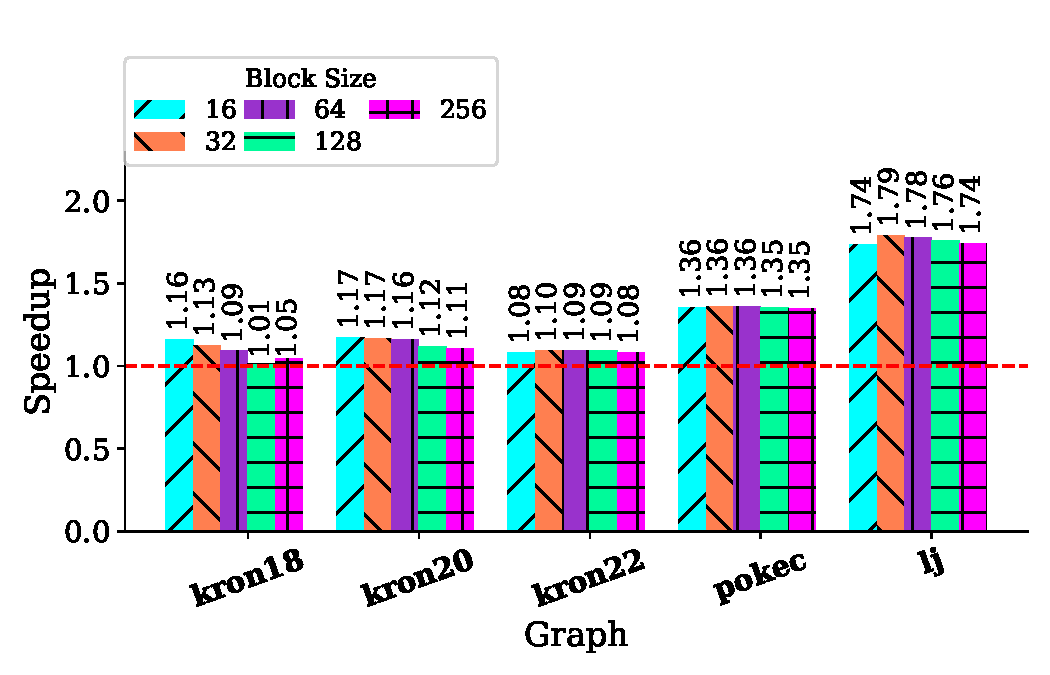
\includegraphics[scale=0.5]{graphit-figures/sssp-cache.pdf}
    \caption{Speedup results for varying work block sizes using the manycore aware vertex partitioning scheme on SSSP. Speedup is calculated over the baseline pull direction implementation.}
    \label{pap:generals:sec:eval:fig:ssspcache}
\end{figure}
 
%\allAlignedFigure
\begin{figure}[t]
    \centering
    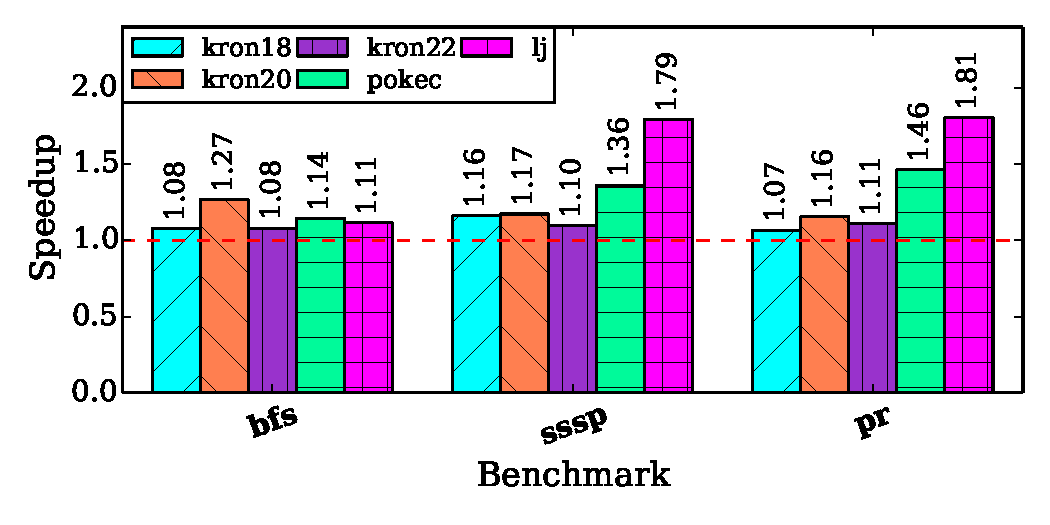
\includegraphics[scale = 0.5]{graphit-figures/align.pdf}
    \caption{Alignment-based partitioning speedup results for each benchmark. Speedup is calculated over the baseline pull direction implementation.} %For each graph and benchmark, work group sizes of 16, 32, 64, 128, and 256 vertices were tested and the best performing work group size is reported here.
    \label{pap:generals:sec:eval:fig:aligned}
    \vspace{-2mm} 
\end{figure}
 
Figure~\ref{pap:generals:sec:eval:fig:ssspcache} shows the performance benefit of alignment-based partitioning across different work block sizes.
Speedup is calculated over the baseline SSSP \pull~implementation. 
Similarly to the blocked access method results, we find that the optimal work block size for alignment-based partitioning is input graph and benchmark dependent. 
A work block size of 16 is optimal for \kron 18 and 20, livejournal and \kron22 see the best performance with a block size of 32, and pokec sees the most speedup with a block size of 64.
 
Figure~\ref{pap:generals:sec:eval:fig:aligned} shows the speedup for each benchmark when using alignment-based partitioning over the baseline vertex partitioning scheme. The optimal work block size for each input graph and benchmark is used to calculate speedup. 
We observe a performance improvement in all input graph and benchmark combinations with an average speedup of 1.25$\times$ and a maximum speedup of 1.8$\times$. 
 
Alignment-based partitioning aims to make better use of the memory system on the manycore. 
By assigning smaller working sets to each core, there is less contention in the LLCs and all benchmarks achieve higher cache hit rates. 
Improving the LLC hit rate decreases the total amount of memory that needs to be read from HBM and decreases the amount of time spent waiting on outstanding memory requests.
 
 
%\edgeSpeedupFigure
\begin{figure}[t]
    \centering
    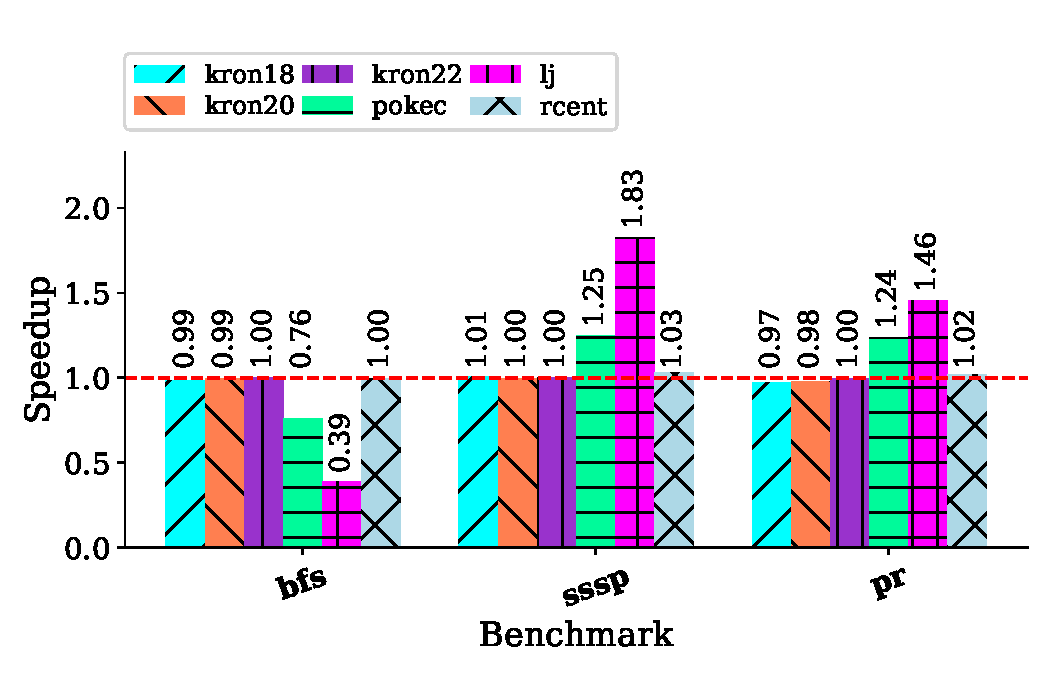
\includegraphics[scale = 0.5]{graphit-figures/edge.pdf}
    \caption{Speedup results for edge based optimization over the baseline dense pull implementation for each benchmark.}
    \label{pap:generals:sec:eval:fig:edge}
    \vspace{-2mm} 
\end{figure}
 
Figure~\ref{pap:generals:sec:eval:fig:edge} shows the performance of edge-aware vertex partitioning relative to the baseline vertex-based partitioning on all benchmarks in the \pull~direction. 
We achieve a speedup in five of the benchmark and input graph combinations with a maximum speedup of 1.5$\times$.
In the cases where performance degraded, we observe an average slowdown 11.7\%. 
This scheduling optimization relies heavily on the structure of the input graph and the algorithm, so these results are somewhat expected.
 
Overall, while we see performance improvements with edge-aware vertex-based partitioning on some benchmarks, we find that alignment-based partitioning provides the most performance improvement in all cases. 
Despite its workload balancing benefits, edge-aware partitioning does not account for the manycore specific properties of the memory system.
Because the memory is the main bottleneck of graph algorithms, the alignment-based scheme which explicitly takes into consideration the properties of the manycore's memory system is ideal. 
 
% \section{Discussion}\label{sec:discussion}
 %\overviewResultsTable
 

% \section{Discussion}\label{sec:discussion}
% %\todo[inline]{(emily) need to reconfigure figure~\ref{fig:overallresults} to group by optimization and by scale of graph (instead of just on optimization like it is now). also need to make sure labels are shown for bars that go above y-axis max}
% \begin{figure}
%     \centering
%     \includegraphics[width=\textwidth]{figures/optimization-speedups_no16.pdf}
%     \caption{Speedups for all of the optimizations we explored in our evaluation. Speedups are calculated over the serial CPU baseline. Speedup is also reported for the parallel CPU implementation over the serial baseline.}
%     \label{fig:overallresults}
% \end{figure}

% Figure~\ref{fig:overallresults} shows an overview of all of the results we presented in Section~\ref{sec:eval}. 
% It shows the speedup for each optimization over the serial CPU baseline in terms of traversed edges per second (TEPS). We observe speedups in 28 of the 30 different cases shown in the figure. We achieve a mean speedup of 3.8$\times$ across optimizations and only see a slowdown of 10\% in the worst case. 

% We see the largest speedups with our blocked \push and blocked \pull implementations.
% This is not surprising, as all of our benchmarks are limited by DRAM, and blocking is an optimization that makes better use of the memory system.
% %This is not surprising, as all of our benchmarks are limited by the memory system performance, and blocking is a memory system optimization.
% By adding blocking, we are able to coalesce read accesses to vertex data, and with the \pull direction, we are also able to batch some of the writes.
% In addition, we able to make use of explicitly managed, low-latency scratchpad memory in our blocked access method. 
% The blocked access method improves the memory system performance of our benchmarks by targeting a key performance limiter of graph algorithms.

% We observe our greatest individual speedups on the \push direction implementations of SSSP. 
% In both the blocked and unblocked implementations, we see very large speedups with the scale 18 graph.
% As noted earlier, SSSP traverses more edges and benefits the most from the prefetching effect of blocking. 
% In the case of the scale 18 \push implementation, we actually observe a slowdown from blocking.
% In this case, the graph must have seen good enough memory system behavior without blocking that the prefetching began to impact performance.

% Again, we note that edge-aware vertex-based partitioning does not have a dramatic impact on performance, but it does outperform the CPU baseline in all cases. 
% This optimization is very input dependent, so we expect that we would see more noticeable improvement with graphs that vary more in structure. 

% We also report the relative performance of the parallel CPU code when compared to the serial CPU code in Figure~\ref{fig:overallresults}.
% We can see that a slowdown is observed in all of the \push benchmarks across all input graphs. 
% We also see a slowdown in three of the nine \pull direction benchmark and input graph combinations.
% We assume that this slowdown is due to the overhead of launching OpenMP threads. 
% Our optimized manycore benchmarks outperform the parallel CPU code in 16 of the 18 cases that we study.
% The parallel CPU code only outperforms our manycore performance on PageRank and SSSP running with the scale 20 input graph. 
% However, we only simulate a small portion of our total manycore architecture. 
% The full manycore architecture would have eight HBM channels instead of the two that we simulate along with many more cores.
% As a result, the full architecture would have much higher memory bandwidth and more compute resources. 
% Because all of our benchmarks are limited by DRAM, we anticipate that we would achieve better performance on the full system due to an increase in memory bandwidth and decrease in memory contention.


\section{Discussion}\label{sec:discussion}
\newcommand{\baselineEvalFigure}{
\begin{figure}[t]
    \centering
    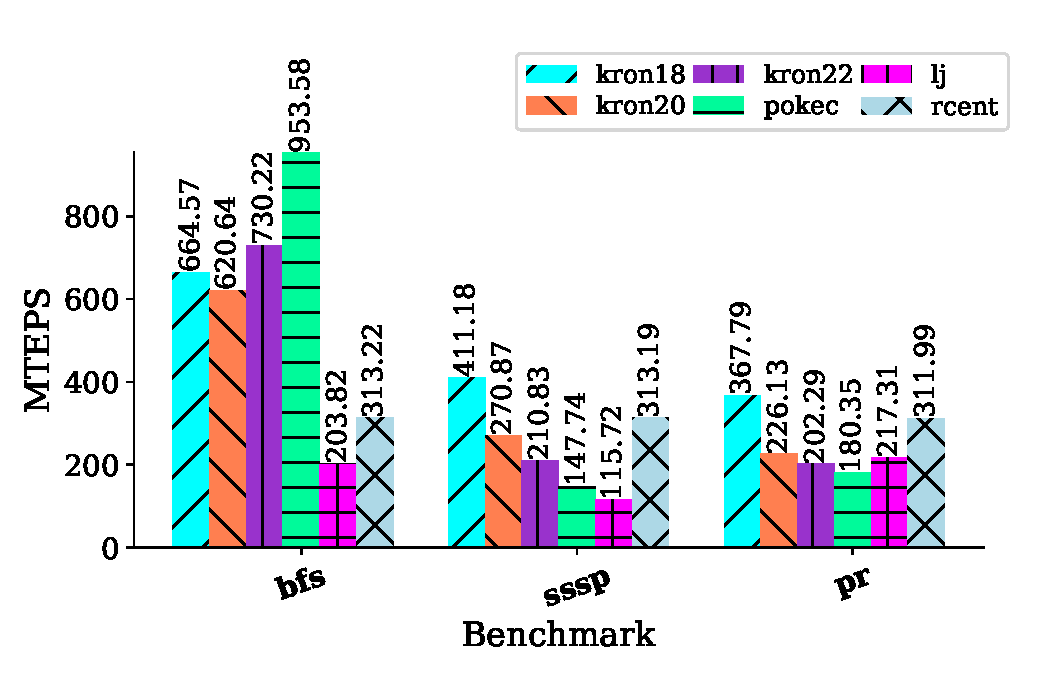
\includegraphics[scale = 0.5]{graphit-figures/baseline.pdf}
    \caption{Baseline code generation results for each benchmark in the dense pull direction with no manycore specific optimizations.}
    \label{pap:generals:sec:eval:fig:baseline}
\end{figure}
}

\newcommand{\pushEvalFigure}{
\begin{figure}[t]
    \centering
    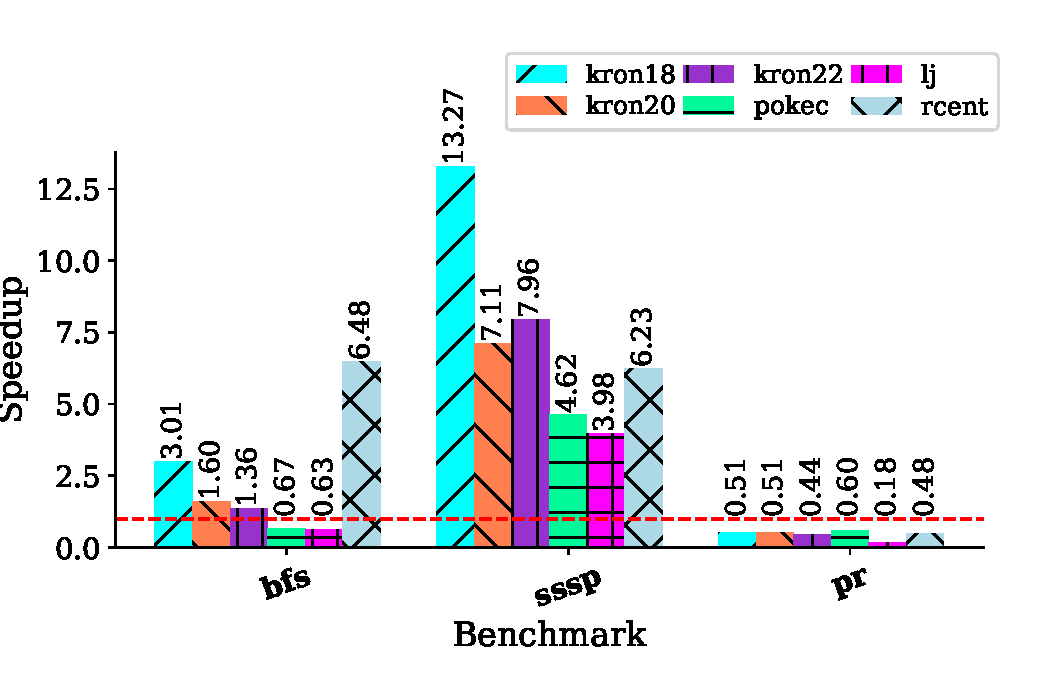
\includegraphics[scale = 0.5]{graphit-figures/push.pdf}
    \caption{Baseline code generation results for each benchmark in the push direction with no manycore specific optimizations.}
    \label{pap:generals:sec:eval:fig:push}
\end{figure}
}

\newcommand{\edgeSpeedupFigure}{
\begin{figure}[t]
    \centering
    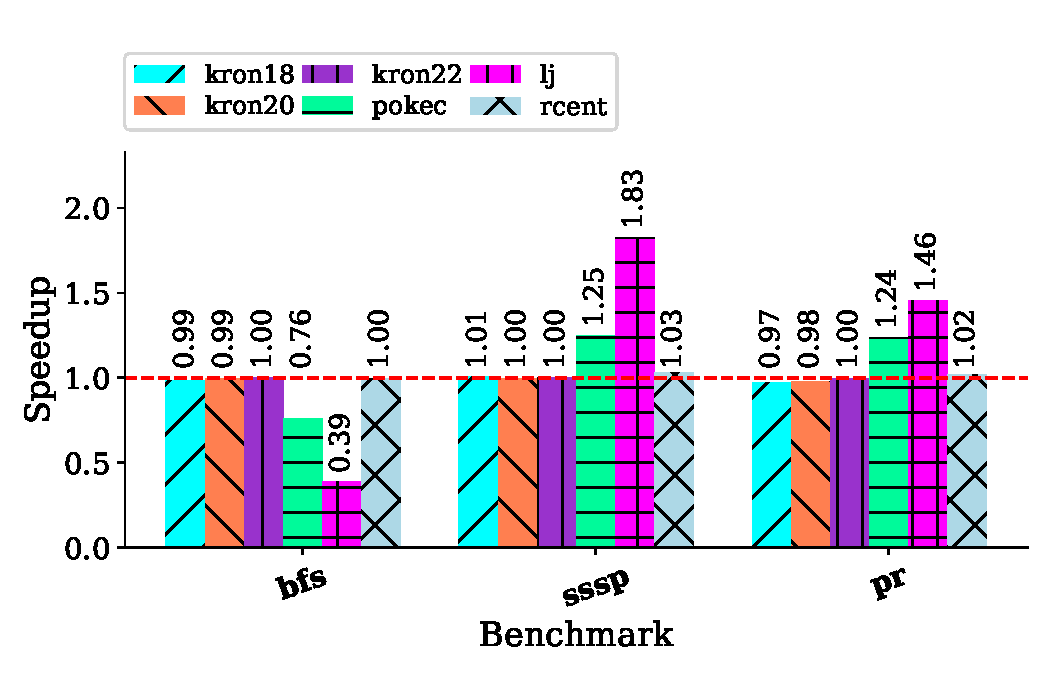
\includegraphics[scale = 0.5]{graphit-figures/edge.pdf}
    \caption{Speedup results for edge based optimization over the baseline dense pull implementation for each benchmark.}
    \label{pap:generals:sec:eval:fig:edge}
    \vspace{-2mm} 
\end{figure}
}

\newcommand{\blockBFSFigure}{
\begin{figure}[t]
    \centering
    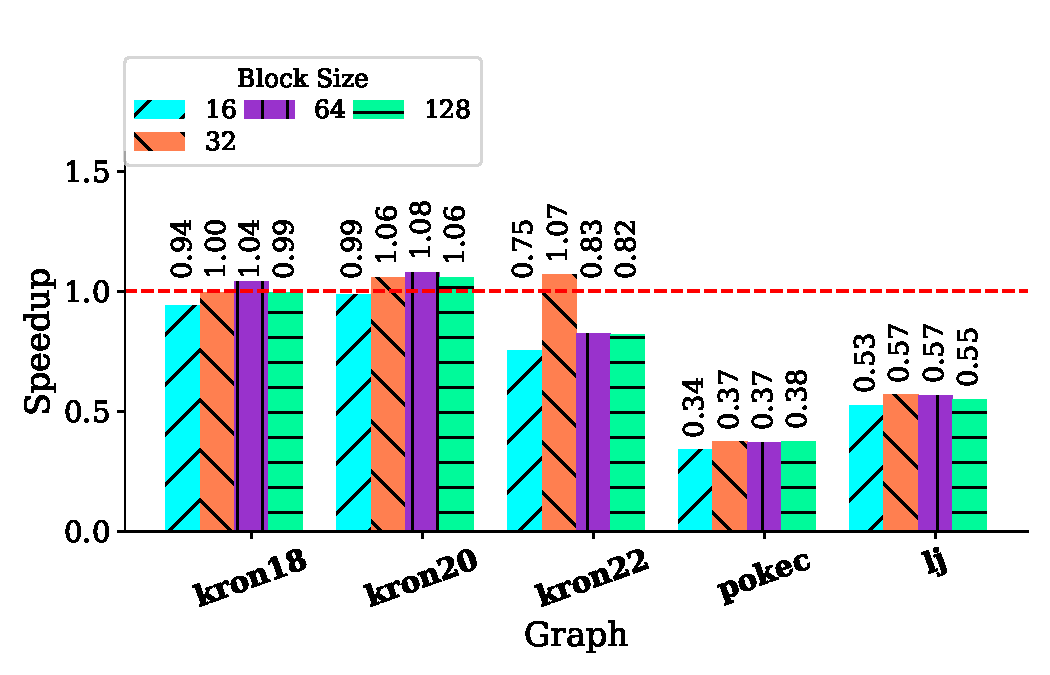
\includegraphics[scale = 0.5]{graphit-figures/bfs-block.pdf}
    \caption{MTEPS results for varying block sizes using the blocked access method on BFS.}
    \label{pap:generals:sec:eval:fig:bfsblock}
\end{figure}
}

\newcommand{\blockSSSPFigure}{
\begin{figure}[t]
    \centering
    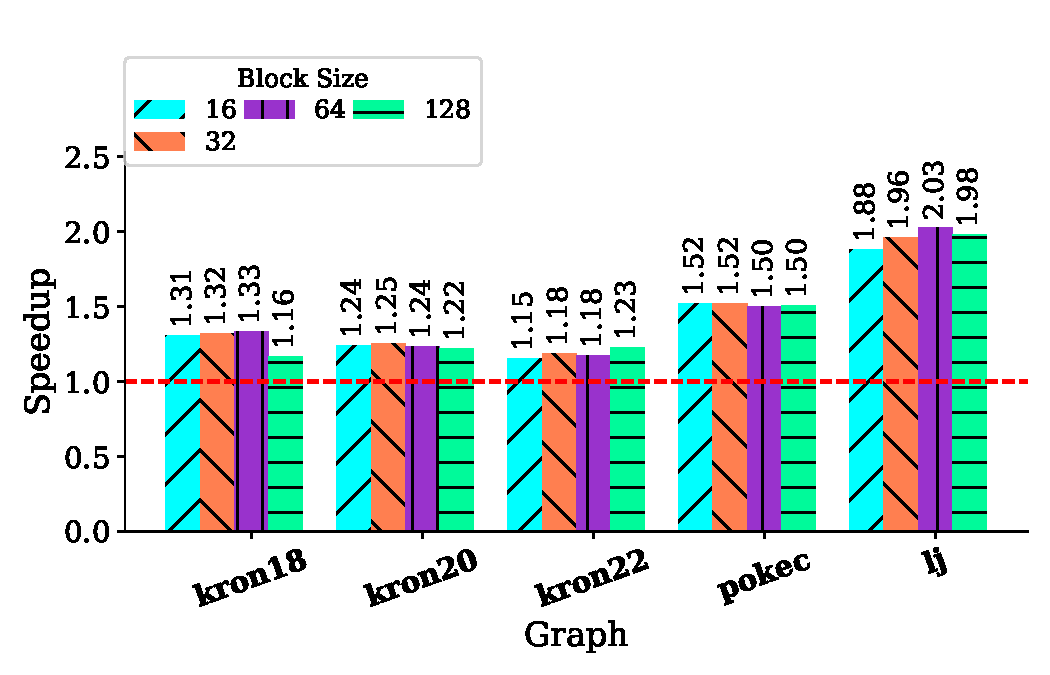
\includegraphics[scale=0.5]{graphit-figures/sssp-block.pdf}
    \caption{Speedup results for varying block sizes using the blocked access method on SSSP. Speedup is calculated over the baseline pull direction implementation.}
    \label{pap:generals:sec:eval:fig:ssspblock}
\end{figure}
}

\newcommand{\cacheBFSFigure}{
\begin{figure}[t]
    \centering
    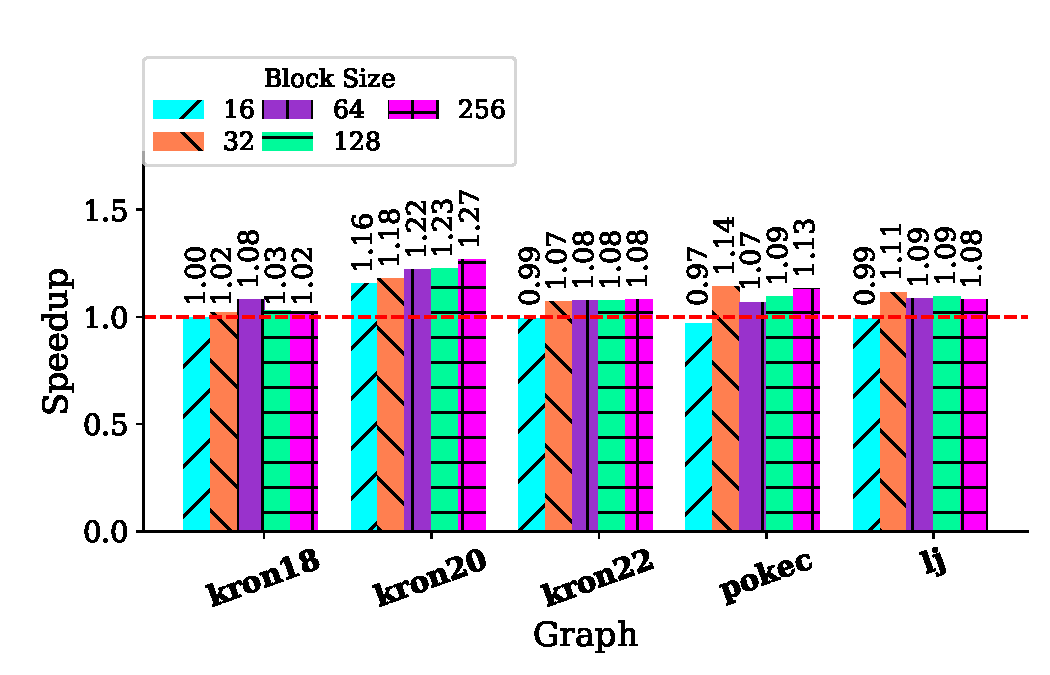
\includegraphics[scale = 0.5]{graphit-figures/bfs-cache.pdf}
    \caption{MTEPS results for varying work block sizes using the manycore aware vertex partitioning scheme on BFS.}
    \label{pap:generals:sec:eval:fig:bfscache}
\end{figure}
}

\newcommand{\cacheSSSPFigure}{
\begin{figure}[t]
    \centering
    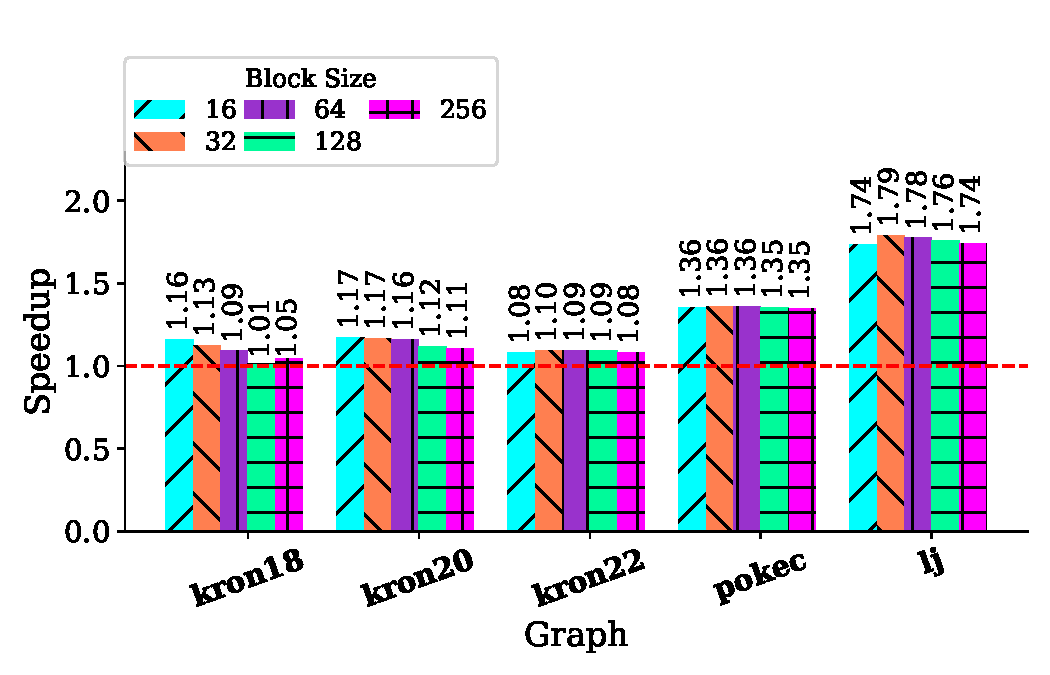
\includegraphics[scale=0.5]{graphit-figures/sssp-cache.pdf}
    \caption{Speedup results for varying work block sizes using the manycore aware vertex partitioning scheme on SSSP. Speedup is calculated over the baseline pull direction implementation.}
    \label{pap:generals:sec:eval:fig:ssspcache}
\end{figure}
}

\newcommand{\allBlockedFigure}{
\begin{figure}[t]
    \centering
    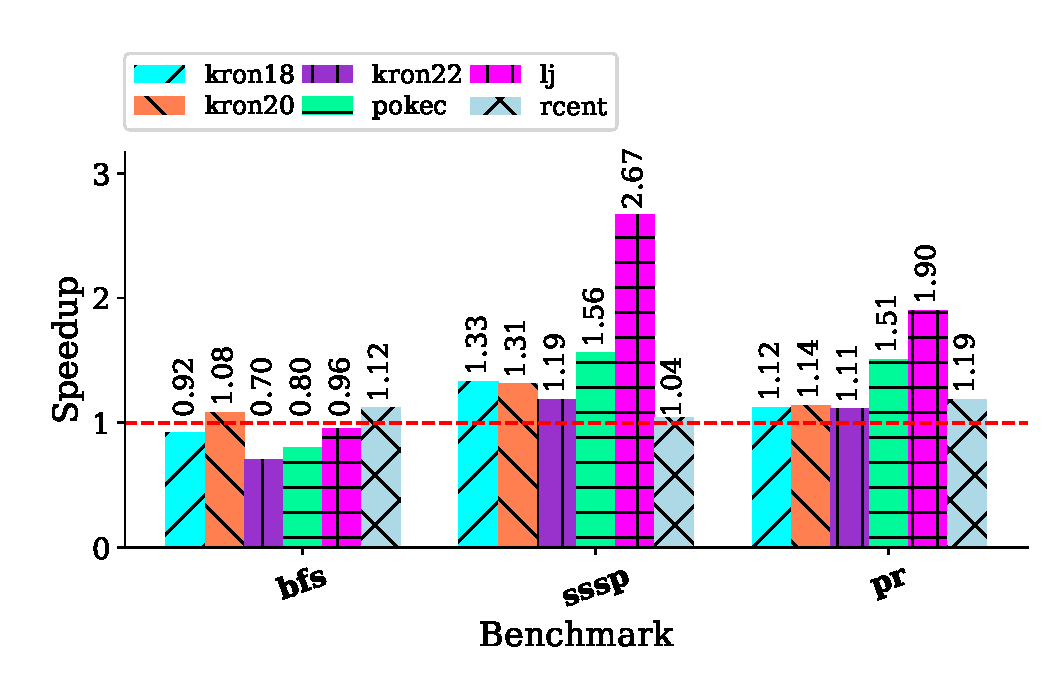
\includegraphics[scale = 0.5]{graphit-figures/all-blocked.pdf}
    \caption{Blocked access method speedup results for each benchmark. Speedup is calculated over the baseline pull direction implementation.} %For each graph and benchmark, block sizes of 16, 32, 64, and 128 elements were tested and the best performing block size is reported here.
    \label{pap:generals:sec:eval:fig:blocked}
\end{figure}
}

\newcommand{\allAlignedFigure}{
\begin{figure}[t]
    \centering
    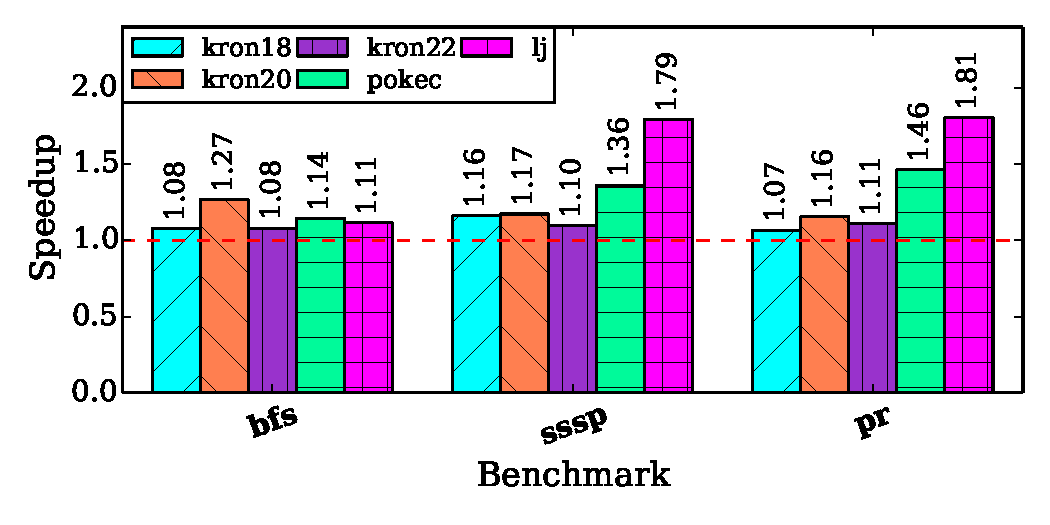
\includegraphics[scale = 0.5]{graphit-figures/align.pdf}
    \caption{Alignment-based partitioning speedup results for each benchmark. Speedup is calculated over the baseline pull direction implementation.} %For each graph and benchmark, work group sizes of 16, 32, 64, 128, and 256 vertices were tested and the best performing work group size is reported here.
    \label{pap:generals:sec:eval:fig:aligned}
    \vspace{-2mm} 
\end{figure}
}

%I am not sure if this is the best way to present an overview of results or if we need it. 
\newcommand{\overviewResultsTable}{
\begin{table}[]
\centering
\begin{tabular}{lrcl}
%\hline
\toprule
\textbf{Benchmark} & \textbf{Graph} & \textbf{MTEPS} & \textbf{Optimization} \\ \midrule
 \multirow{5}{*}{BFS}& kron18 & 457.09 & Cache-Aligned \pull \\ %\cline{2-4}
 & kron20 & 296.32 & Cache-Aligned \pull \\ %cline{2-4}
 & kron22 & 241.95 & Cache-Aligned \pull \\ %\cline{2-4}
 & pokec & 148.02 &  Cache-Aligned \pull\\ %\cline{2-4}
 & lj & 304.36 & Cache-Aligned \pull \\ \hline
 \multirow{5}{*}{PR}& kron18 & 412.34 & Blocked \pull \\ %\cline{2-4}
 & kron20 & 261.35 & Cache-Aligned \pull \\ %\cline{2-4}
 & kron22 & 224.88 & Blocked \pull \\ %\cline{2-4}
 & pokec & 272.57 & Blocked \pull \\ %\cline{2-4}
 & lj & 413.06 & Blocked \pull \\ \hline
 \multirow{5}{*}{SSSP}& kron18 & 467.08 & Cache-Aligned \pull \\ %\cline{2-4}
 & kron20 & 364.36& Baseline \push \\ %\cline{2-4}
 & kron22 & 404.27 & Baseline \push \\ %\cline{2-4}
 & pokec & 149.17 & Cache-Aligned \pull \\ %\cline{2-4}
 & lj & 268.87 & Cache-Aligned \pull \\ %\hline
 \bottomrule
\end{tabular}
\caption{Table containing best MTEPS results across all benchmarks and input graphs. The optimizations used to achieve these results are also listed above.}
\label{pap:generals:sec:eval:tab:overview}
\end{table}
}

\newcommand{\relatedMTEPSTable}{
\begin{table}[]
\centering
\begin{tabular}{cllll}
%\hline
\toprule
 \textbf{Source} & \textbf{Platform} & \textbf{Benchmark} & \textbf{Graph}  & \textbf{MTEPS} \\ \midrule
 \cite{slota2015high}& Xeon Phi MIC & CC & LJ (22) & 240 \\ %\hline
 \cite{slota2015high}& Xeon Phi MIC & CC & Flickr (19) & 140\\ %\hline
 %Galois \cite{aasawat2018well}& Ivy Bridge & PR & LJ (22) & 207.67 \\ \hline
 \cite{khorasani2014cusha} & GTX780 & BFS & LJ (22) & 272.4 \\ %\hline
 \cite{zhong2013medusa}& C2050 & BFS & KKT (21) & 351.5 \\ %\hline
 \cite{yang2019graphblast}& k40c & SSSP & LJ (22) & 334.2 \\ %\hline
 \cite{wang2016gunrock} & k40c & SSSP & LJ (22) & 217.9 \\
 \bottomrule

\end{tabular}
\caption{Performance results in MTEPS from other graph processing frameworks. The benchmark CC is strongly connected components.}
\label{sec:related:tab:mteps}
\vspace{-1mm} 
\end{table}
}
\newcommand{\graphInfoTable}{
\begin{table}[]
\centering
\begin{tabular}{c|c|c|c}
%\hline
 \textbf{Name} & \textbf{Scale} & \textbf{\# Vertices} & \textbf{\# Edges} \\ \hline %\hline
 kron18 & 18 & 262,144 & 4,194,304 \\ \hline
 kron20 & 20 & 1,048,576 & 16,777,216 \\ \hline
 kron22 & 22 & 4,194,304 & 67,108,864 \\ \hline
 pokec & 20.5 & 1,632,803 & 30,622,564 \\ \hline
 livejournal (lj) & 22 & 3,997,962 & 34,681,189 \\ %\hline
\end{tabular}

\caption{The vertex and edge information for each of the graphs used in our evaluation. We use synthetic \kron graphs used in the Graph500 benchmark and two real world graphs.}
\label{sec:eval:tab:graphs}
\end{table}
}

\begin{figure}[t!]
    \centering
    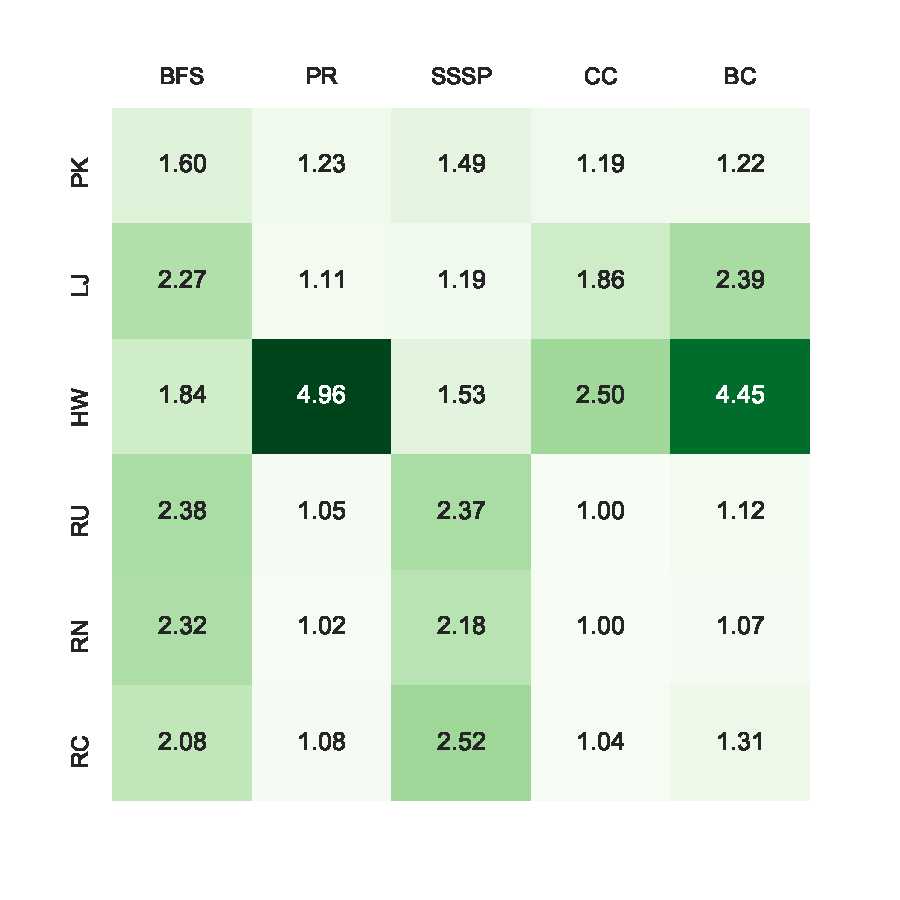
\includegraphics[scale=0.6]{graphit-figures/heatmap.pdf}
    \caption{Speedups for all benchmarks and real-world input graphs attained from applying the blocked-access method or alignment-based partitioning optimization. Here we examine BFS, PR, CC, BC, and the delta-stepping variant of SSSP.}
    \label{pap:generals:sec:eval:fig:heatmap}
\end{figure}

Figure~\ref{pap:generals:sec:eval:fig:heatmap} shows speedups obtained from applying the blocked-access method or alignment-based partitioning to a wider range of benchmarks and input graphs.
Here we evaluate performance on three real-world social network graphs (Livejournal, pokec, and Hollywood) and three road networks (RoadCA, RoadCentral, and RoadUSA).
In addition to BFS and PR we also evaluate on SSSP with delta-stepping, CC, and BC.
%Due to the costs of RTL simulation, we evaluate the \hbvm on 6 of the 10 input graphs and a subset of the total iterations for each application.
For PR we simulate one iteration, and for the remaining applications, we simulate five representative iterations that cover a range of frontier densities and execution behavior.
We use hybrid traversal in the baseline code of BFS, BC, and SSSP to decrease simulation times.
%The speedups reported in Figure~\ref{base_v_opt} come from applying the \hbmc-specific optimizations described in Section~\ref{sec:compilerimpl:hbvm}.
BC, CC, and BFS benefit from alignment-based partitioning, while PR and SSSP use the blocking optimization due to their more compute-intensive nature.
As shown throughout our evaluation, these optimizations better utilize the memory hierarchy and provide up to $4.96\times$ speedup over unoptimized code.

Table~\ref{sec:eval:tab:summary} shows the highest achieved MTEPS for each input graph and benchmark along with the optimization that was used in the generated code.
Alignment-based partitioning provides optimal performance across the most input graphs and benchmarks, and the next best performing optimization is blocking.
This is not surprising, as all of our benchmarks are limited by DRAM, and blocking and alignment-based partitioning are optimizations that makes better use of the memory system.
By adding blocking and alignment-based partitioning, we are able to coalesce read accesses to vertex data.
In addition, with blocking, we are able to make use of explicitly managed, low-latency scratchpad memory in our blocked access method. 
The blocked access method and alignment-based partitioning improve the memory system performance of our benchmarks by targeting a key performance limiter of graph algorithms.

\relatedMTEPSTable

We do not include a direct comparison of our results against other systems; however, Table~\ref{sec:related:tab:mteps} shows performance for some of the frameworks mentioned in Chapter~\ref{gen:sec:background}. This table is included to help contextualize the results reported above.
% We only include results from the papers that report performance in MTEPS. We include this table to help contextualize our results.
It is also important to note that we only simulate a small portion of the total manycore architecture. 
The full manycore architecture would have eight HBM channels instead of the two that are simulated along with many more cores.
As a result, the full architecture would have much higher memory bandwidth and more compute resources. 
Because all of our benchmarks are limited by DRAM, we anticipate that we would achieve better performance on the full system due to an increase in memory bandwidth and decrease in memory contention.

\overviewResultsTable
\subsection{Conclusions}\label{sec:concl}

In this section, we presented our work developing a code generator for graph processing frameworks targeting a representative manycore architecture. 
We formalized a general execution model and presented a backend that supports code generation for this model on a manycore architecture that utilizes High Bandwidth Memory.
We proposed two manycore specific optimizations to improve performance across graph programs, and showed how existing graph processing optimizations can be ported to a manycore. 
A performance study found that our optimized manycore code achieves 467 million traversed edges per second (MTEPS) exceeding conventional architectures in a fraction of the die area.

%\todo{more conclusion here? paragraph on the impact/future implications?}

% Code generation offers us the ability to abstract away the complexity of writing performant manycore code from the specification of the graph application. 
% The \graphit DSL further allows us to more easily explore ways to improve performance across benchmarks and input graphs by separating the algorithm description from the scheduling of work.

